% Options for packages loaded elsewhere
\PassOptionsToPackage{unicode}{hyperref}
\PassOptionsToPackage{hyphens}{url}
\PassOptionsToPackage{dvipsnames,svgnames,x11names}{xcolor}
%
\documentclass[
  letterpaper,
  DIV=11,
  numbers=noendperiod]{scrartcl}

\usepackage{amsmath,amssymb}
\usepackage{iftex}
\ifPDFTeX
  \usepackage[T1]{fontenc}
  \usepackage[utf8]{inputenc}
  \usepackage{textcomp} % provide euro and other symbols
\else % if luatex or xetex
  \usepackage{unicode-math}
  \defaultfontfeatures{Scale=MatchLowercase}
  \defaultfontfeatures[\rmfamily]{Ligatures=TeX,Scale=1}
\fi
\usepackage{lmodern}
\ifPDFTeX\else  
    % xetex/luatex font selection
\fi
% Use upquote if available, for straight quotes in verbatim environments
\IfFileExists{upquote.sty}{\usepackage{upquote}}{}
\IfFileExists{microtype.sty}{% use microtype if available
  \usepackage[]{microtype}
  \UseMicrotypeSet[protrusion]{basicmath} % disable protrusion for tt fonts
}{}
\makeatletter
\@ifundefined{KOMAClassName}{% if non-KOMA class
  \IfFileExists{parskip.sty}{%
    \usepackage{parskip}
  }{% else
    \setlength{\parindent}{0pt}
    \setlength{\parskip}{6pt plus 2pt minus 1pt}}
}{% if KOMA class
  \KOMAoptions{parskip=half}}
\makeatother
\usepackage{xcolor}
\setlength{\emergencystretch}{3em} % prevent overfull lines
\setcounter{secnumdepth}{-\maxdimen} % remove section numbering
% Make \paragraph and \subparagraph free-standing
\makeatletter
\ifx\paragraph\undefined\else
  \let\oldparagraph\paragraph
  \renewcommand{\paragraph}{
    \@ifstar
      \xxxParagraphStar
      \xxxParagraphNoStar
  }
  \newcommand{\xxxParagraphStar}[1]{\oldparagraph*{#1}\mbox{}}
  \newcommand{\xxxParagraphNoStar}[1]{\oldparagraph{#1}\mbox{}}
\fi
\ifx\subparagraph\undefined\else
  \let\oldsubparagraph\subparagraph
  \renewcommand{\subparagraph}{
    \@ifstar
      \xxxSubParagraphStar
      \xxxSubParagraphNoStar
  }
  \newcommand{\xxxSubParagraphStar}[1]{\oldsubparagraph*{#1}\mbox{}}
  \newcommand{\xxxSubParagraphNoStar}[1]{\oldsubparagraph{#1}\mbox{}}
\fi
\makeatother

\usepackage{color}
\usepackage{fancyvrb}
\newcommand{\VerbBar}{|}
\newcommand{\VERB}{\Verb[commandchars=\\\{\}]}
\DefineVerbatimEnvironment{Highlighting}{Verbatim}{commandchars=\\\{\}}
% Add ',fontsize=\small' for more characters per line
\usepackage{framed}
\definecolor{shadecolor}{RGB}{241,243,245}
\newenvironment{Shaded}{\begin{snugshade}}{\end{snugshade}}
\newcommand{\AlertTok}[1]{\textcolor[rgb]{0.68,0.00,0.00}{#1}}
\newcommand{\AnnotationTok}[1]{\textcolor[rgb]{0.37,0.37,0.37}{#1}}
\newcommand{\AttributeTok}[1]{\textcolor[rgb]{0.40,0.45,0.13}{#1}}
\newcommand{\BaseNTok}[1]{\textcolor[rgb]{0.68,0.00,0.00}{#1}}
\newcommand{\BuiltInTok}[1]{\textcolor[rgb]{0.00,0.23,0.31}{#1}}
\newcommand{\CharTok}[1]{\textcolor[rgb]{0.13,0.47,0.30}{#1}}
\newcommand{\CommentTok}[1]{\textcolor[rgb]{0.37,0.37,0.37}{#1}}
\newcommand{\CommentVarTok}[1]{\textcolor[rgb]{0.37,0.37,0.37}{\textit{#1}}}
\newcommand{\ConstantTok}[1]{\textcolor[rgb]{0.56,0.35,0.01}{#1}}
\newcommand{\ControlFlowTok}[1]{\textcolor[rgb]{0.00,0.23,0.31}{\textbf{#1}}}
\newcommand{\DataTypeTok}[1]{\textcolor[rgb]{0.68,0.00,0.00}{#1}}
\newcommand{\DecValTok}[1]{\textcolor[rgb]{0.68,0.00,0.00}{#1}}
\newcommand{\DocumentationTok}[1]{\textcolor[rgb]{0.37,0.37,0.37}{\textit{#1}}}
\newcommand{\ErrorTok}[1]{\textcolor[rgb]{0.68,0.00,0.00}{#1}}
\newcommand{\ExtensionTok}[1]{\textcolor[rgb]{0.00,0.23,0.31}{#1}}
\newcommand{\FloatTok}[1]{\textcolor[rgb]{0.68,0.00,0.00}{#1}}
\newcommand{\FunctionTok}[1]{\textcolor[rgb]{0.28,0.35,0.67}{#1}}
\newcommand{\ImportTok}[1]{\textcolor[rgb]{0.00,0.46,0.62}{#1}}
\newcommand{\InformationTok}[1]{\textcolor[rgb]{0.37,0.37,0.37}{#1}}
\newcommand{\KeywordTok}[1]{\textcolor[rgb]{0.00,0.23,0.31}{\textbf{#1}}}
\newcommand{\NormalTok}[1]{\textcolor[rgb]{0.00,0.23,0.31}{#1}}
\newcommand{\OperatorTok}[1]{\textcolor[rgb]{0.37,0.37,0.37}{#1}}
\newcommand{\OtherTok}[1]{\textcolor[rgb]{0.00,0.23,0.31}{#1}}
\newcommand{\PreprocessorTok}[1]{\textcolor[rgb]{0.68,0.00,0.00}{#1}}
\newcommand{\RegionMarkerTok}[1]{\textcolor[rgb]{0.00,0.23,0.31}{#1}}
\newcommand{\SpecialCharTok}[1]{\textcolor[rgb]{0.37,0.37,0.37}{#1}}
\newcommand{\SpecialStringTok}[1]{\textcolor[rgb]{0.13,0.47,0.30}{#1}}
\newcommand{\StringTok}[1]{\textcolor[rgb]{0.13,0.47,0.30}{#1}}
\newcommand{\VariableTok}[1]{\textcolor[rgb]{0.07,0.07,0.07}{#1}}
\newcommand{\VerbatimStringTok}[1]{\textcolor[rgb]{0.13,0.47,0.30}{#1}}
\newcommand{\WarningTok}[1]{\textcolor[rgb]{0.37,0.37,0.37}{\textit{#1}}}

\providecommand{\tightlist}{%
  \setlength{\itemsep}{0pt}\setlength{\parskip}{0pt}}\usepackage{longtable,booktabs,array}
\usepackage{calc} % for calculating minipage widths
% Correct order of tables after \paragraph or \subparagraph
\usepackage{etoolbox}
\makeatletter
\patchcmd\longtable{\par}{\if@noskipsec\mbox{}\fi\par}{}{}
\makeatother
% Allow footnotes in longtable head/foot
\IfFileExists{footnotehyper.sty}{\usepackage{footnotehyper}}{\usepackage{footnote}}
\makesavenoteenv{longtable}
\usepackage{graphicx}
\makeatletter
\def\maxwidth{\ifdim\Gin@nat@width>\linewidth\linewidth\else\Gin@nat@width\fi}
\def\maxheight{\ifdim\Gin@nat@height>\textheight\textheight\else\Gin@nat@height\fi}
\makeatother
% Scale images if necessary, so that they will not overflow the page
% margins by default, and it is still possible to overwrite the defaults
% using explicit options in \includegraphics[width, height, ...]{}
\setkeys{Gin}{width=\maxwidth,height=\maxheight,keepaspectratio}
% Set default figure placement to htbp
\makeatletter
\def\fps@figure{htbp}
\makeatother

\usepackage{fvextra}
\DefineVerbatimEnvironment{Highlighting}{Verbatim}{breaklines,commandchars=\\\{\}}
\KOMAoption{captions}{tableheading}
\usepackage{multicol}
\newcommand{\btwocol}{\begin{multicols}{2}}
\newcommand{\etwocol}{\end{multicols}}
\makeatletter
\@ifpackageloaded{caption}{}{\usepackage{caption}}
\AtBeginDocument{%
\ifdefined\contentsname
  \renewcommand*\contentsname{Table of contents}
\else
  \newcommand\contentsname{Table of contents}
\fi
\ifdefined\listfigurename
  \renewcommand*\listfigurename{List of Figures}
\else
  \newcommand\listfigurename{List of Figures}
\fi
\ifdefined\listtablename
  \renewcommand*\listtablename{List of Tables}
\else
  \newcommand\listtablename{List of Tables}
\fi
\ifdefined\figurename
  \renewcommand*\figurename{Figure}
\else
  \newcommand\figurename{Figure}
\fi
\ifdefined\tablename
  \renewcommand*\tablename{Table}
\else
  \newcommand\tablename{Table}
\fi
}
\@ifpackageloaded{float}{}{\usepackage{float}}
\floatstyle{ruled}
\@ifundefined{c@chapter}{\newfloat{codelisting}{h}{lop}}{\newfloat{codelisting}{h}{lop}[chapter]}
\floatname{codelisting}{Listing}
\newcommand*\listoflistings{\listof{codelisting}{List of Listings}}
\makeatother
\makeatletter
\makeatother
\makeatletter
\@ifpackageloaded{caption}{}{\usepackage{caption}}
\@ifpackageloaded{subcaption}{}{\usepackage{subcaption}}
\makeatother

\ifLuaTeX
  \usepackage{selnolig}  % disable illegal ligatures
\fi
\usepackage{bookmark}

\IfFileExists{xurl.sty}{\usepackage{xurl}}{} % add URL line breaks if available
\urlstyle{same} % disable monospaced font for URLs
\hypersetup{
  pdftitle={CS/DS 541: Deep Learning},
  colorlinks=true,
  linkcolor={blue},
  filecolor={Maroon},
  citecolor={Blue},
  urlcolor={Blue},
  pdfcreator={LaTeX via pandoc}}


\title{CS/DS 541: Deep Learning}
\usepackage{etoolbox}
\makeatletter
\providecommand{\subtitle}[1]{% add subtitle to \maketitle
  \apptocmd{\@title}{\par {\large #1 \par}}{}{}
}
\makeatother
\subtitle{Homework 2}
\author{}
\date{}

\begin{document}
\maketitle

\RecustomVerbatimEnvironment{verbatim}{Verbatim}{
  showspaces = false,
  showtabs = false,
  breaksymbolleft={},
  breaklines
  % Note: setting commandchars=\\\{\} here will cause an error
}


\textbf{Due: 5:59pm ET Thursday September 18}

This problem can be done in teams of up 2 students.

\begin{center}\rule{0.5\linewidth}{0.5pt}\end{center}

\subsection{Problem 1: Derivation of softmax regression gradient {[}15
points{]}}\label{problem-1-derivation-of-softmax-regression-gradient-15-points}

As explained in class, the softmax regression generalizes the logistic
regression to multi-class classification. Let

\[
W = 
\begin{bmatrix}
w^{(1)} \ \ldots \ w^{(c)}
\end{bmatrix}
\]

be an \(m \times c\) matrix containing the weight vectors from the \(c\)
different classes. The output of the softmax regression neural network
is a vector with \(c\) dimensions such that:

\[
\hat{y}_k = \frac{\exp(z_k)}{\sum_{k'=1}^c \exp(z_{k'})} \tag{0.0.1}
\]

\[
z_k = x^\top w^{(k)} + b_k
\]

for each \(k = 1, \ldots, c\). Correspondingly, our cost function will
sum over all \(c\) classes:

\[
f_{CE}(W,b) = -\frac{1}{n} \sum_{i=1}^n \sum_{k=1}^c y_k^{(i)} \log \hat{y}_k^{(i)}
\]

\begin{center}\rule{0.5\linewidth}{0.5pt}\end{center}

\textbf{Important note:} When deriving the gradient expression for each
weight vector \(w^{(l)}\), it is crucial to keep in mind that the weight
vector for each class \(l \in \{1, \ldots, c\}\) affects the outputs of
the network for every class, not just for class \(l\). This is due to
the normalization in Equation 0.0.1 -- if changing the weight vector
increases the value of \(\hat{y}_l\), then it necessarily must decrease
the values of the other \(\hat{y}_{l' \neq l}\).

\begin{center}\rule{0.5\linewidth}{0.5pt}\end{center}

In this homework problem, please complete the following derivation that
is outlined below:

Derivation: For each weight vector \(w^{(l)}\), we can derive the
gradient expression as:

\[
\nabla_{w^{(l)}} f_{CE}(W,b) = -\frac{1}{n} \sum_{i=1}^n \sum_{k=1}^c y_k^{(i)} \nabla_{w^{(l)}} \log \hat{y}_k^{(i)}
\]

\[
= -\frac{1}{n} \sum_{i=1}^n \sum_{k=1}^c y_k^{(i)} \left( \frac{\nabla_{w^{(l)}} \hat{y}_k^{(i)}}{\hat{y}_k^{(i)}} \right)
\]

\begin{center}\rule{0.5\linewidth}{0.5pt}\end{center}

We handle the two cases \(l = k\) and \(l \neq k\) separately.

For \(l = k\):

\[
\nabla_{w^{(l)}} \hat{y}_k^{(i)} = \text{complete me...}
\]

\[
= x^{(i)} \hat{y}_l^{(i)} (1 - \hat{y}_l^{(i)})
\]

For \(l \neq k\):

\[
\nabla_{w^{(l)}} \hat{y}_k^{(i)} = \text{complete me...}
\]

\[
= -x^{(i)} \hat{y}_k^{(i)} \hat{y}_l^{(i)}
\]

\begin{center}\rule{0.5\linewidth}{0.5pt}\end{center}

To compute the total gradient of \(f_{CE}\) w.r.t. each \(w^{(k)}\), we
have to sum over all examples and over \(l = 1, \ldots, c\). (Hint:
\(\sum_k a_k = a_l + \sum_{k \neq l} a_k.\) Also, \(\sum_k y_k = 1.\))

\[
\nabla_{w^{(l)}} f_{CE}(W,b) = -\frac{1}{n} \sum_{i=1}^n \sum_{k=1}^c y_k^{(i)} \nabla_{w^{(l)}} \log \hat{y}_k^{(i)}
\]

\[
= \text{complete me...}
\]

\[
= -\frac{1}{n} \sum_{i=1}^n x^{(i)} \left( y_l^{(i)} - \hat{y}_l^{(i)} \right)
\]

\begin{center}\rule{0.5\linewidth}{0.5pt}\end{center}

Finally, show that:

\[
\nabla_b f_{CE}(W,b) = -\frac{1}{n} \sum_{i=1}^n \left( y^{(i)} - \hat{y}^{(i)} \right)
\]

\begin{center}\rule{0.5\linewidth}{0.5pt}\end{center}

\subsubsection{Answers:}\label{answers}

Step 1 \(\nabla_{\mathbf{w}^{(l)}} \hat{y}_k^{(i)}\)

\[\nabla_{\mathbf{w}^{(l)}} \hat{y}_k^{(i)} = \frac{\partial \hat{y}_k^{(i)}}{\partial z_l^{(i)}} \cdot \frac{\partial z_l^{(i)}}{\partial \mathbf{w}^{(l)}} \quad \text{(chain rule)}\]

\[\frac{\partial z_l^{(i)}}{\partial \mathbf{w}^{(l)}} = \frac{\partial}{\partial \mathbf{w}^{(l)}}[(\mathbf{x}^{(i)})^T \mathbf{w}^{(l)} + b_l] = \mathbf{x}^{(i)} \in \mathbb{R}^m \quad \text{(}\nabla_{\mathbf{w}}[\mathbf{a}^T\mathbf{w}] = \mathbf{a}\text{)}\]

Case \(l = k\)

\[\frac{\partial \hat{y}_k^{(i)}}{\partial z_k^{(i)}} = \frac{\partial}{\partial z_k^{(i)}}\left[\frac{\exp(z_k^{(i)})}{\sum_{k'=1}^c \exp(z_{k'}^{(i)})}\right]\]

\[= \frac{\exp(z_k^{(i)}) \cdot \sum_{k'=1}^c \exp(z_{k'}^{(i)}) - \exp(z_k^{(i)}) \cdot \exp(z_k^{(i)})}{[\sum_{k'=1}^c \exp(z_{k'}^{(i)})]^2} \quad \left(\frac{d}{dx}\left[\frac{f}{g}\right] = \frac{f'g - fg'}{g^2}\right)\]

\[= \frac{\exp(z_k^{(i)}) \cdot [\sum_{k'=1}^c \exp(z_{k'}^{(i)}) - \exp(z_k^{(i)})]}{[\sum_{k'=1}^c \exp(z_{k'}^{(i)})]^2}\]

\[= \frac{\exp(z_k^{(i)})}{\sum_{k'=1}^c \exp(z_{k'}^{(i)})} \cdot \frac{\sum_{k'=1}^c \exp(z_{k'}^{(i)}) - \exp(z_k^{(i)})}{\sum_{k'=1}^c \exp(z_{k'}^{(i)})}\]

\[= \hat{y}_k^{(i)} \cdot \left(1 - \frac{\exp(z_k^{(i)})}{\sum_{k'=1}^c \exp(z_{k'}^{(i)})}\right)\]

\[= \hat{y}_k^{(i)}(1 - \hat{y}_k^{(i)})\]

\[\therefore \nabla_{\mathbf{w}^{(k)}} \hat{y}_k^{(i)} = \mathbf{x}^{(i)} \hat{y}_k^{(i)}(1 - \hat{y}_k^{(i)}) \in \mathbb{R}^m\]

Case \(l \neq k\)

\[\frac{\partial \hat{y}_k^{(i)}}{\partial z_l^{(i)}} = \frac{\partial}{\partial z_l^{(i)}}\left[\frac{\exp(z_k^{(i)})}{\sum_{k'=1}^c \exp(z_{k'}^{(i)})}\right]\]

\[= \frac{0 \cdot \sum_{k'=1}^c \exp(z_{k'}^{(i)}) - \exp(z_k^{(i)}) \cdot \exp(z_l^{(i)})}{[\sum_{k'=1}^c \exp(z_{k'}^{(i)})]^2} \quad \left(\frac{\partial \exp(z_k)}{\partial z_l} = 0, \; k \neq l\right)\]

\[= -\frac{\exp(z_k^{(i)}) \cdot \exp(z_l^{(i)})}{[\sum_{k'=1}^c \exp(z_{k'}^{(i)})]^2}\]

\[= -\frac{\exp(z_k^{(i)})}{\sum_{k'=1}^c \exp(z_{k'}^{(i)})} \cdot \frac{\exp(z_l^{(i)})}{\sum_{k'=1}^c \exp(z_{k'}^{(i)})}\]

\[= -\hat{y}_k^{(i)} \hat{y}_l^{(i)}\]

\[\therefore \nabla_{\mathbf{w}^{(l)}} \hat{y}_k^{(i)} = -\mathbf{x}^{(i)} \hat{y}_k^{(i)} \hat{y}_l^{(i)} \in \mathbb{R}^m\]

Step 2 \(\nabla_{\mathbf{w}^{(l)}} f_{CE}\)

\[\nabla_{\mathbf{w}^{(l)}} f_{CE} = -\frac{1}{n}\sum_{i=1}^n\sum_{k=1}^c y_k^{(i)} \nabla_{\mathbf{w}^{(l)}} \log \hat{y}_k^{(i)}\]

\[= -\frac{1}{n}\sum_{i=1}^n\sum_{k=1}^c y_k^{(i)} \cdot \frac{1}{\hat{y}_k^{(i)}} \cdot \nabla_{\mathbf{w}^{(l)}} \hat{y}_k^{(i)} \quad \left(\frac{d}{dx}\log f = \frac{1}{f} \cdot \frac{df}{dx}\right)\]

\[= -\frac{1}{n}\sum_{i=1}^n\left[\sum_{k=1}^c y_k^{(i)} \cdot \frac{\nabla_{\mathbf{w}^{(l)}} \hat{y}_k^{(i)}}{\hat{y}_k^{(i)}}\right]\]

\[= -\frac{1}{n}\sum_{i=1}^n\left[y_l^{(i)} \cdot \frac{\nabla_{\mathbf{w}^{(l)}} \hat{y}_l^{(i)}}{\hat{y}_l^{(i)}} + \sum_{k \neq l} y_k^{(i)} \cdot \frac{\nabla_{\mathbf{w}^{(l)}} \hat{y}_k^{(i)}}{\hat{y}_k^{(i)}}\right]\]

\[= -\frac{1}{n}\sum_{i=1}^n\left[y_l^{(i)} \cdot \frac{\mathbf{x}^{(i)} \hat{y}_l^{(i)}(1 - \hat{y}_l^{(i)})}{\hat{y}_l^{(i)}} + \sum_{k \neq l} y_k^{(i)} \cdot \frac{-\mathbf{x}^{(i)} \hat{y}_k^{(i)} \hat{y}_l^{(i)}}{\hat{y}_k^{(i)}}\right]\]

\[= -\frac{1}{n}\sum_{i=1}^n\left[\mathbf{x}^{(i)} y_l^{(i)} (1 - \hat{y}_l^{(i)}) - \mathbf{x}^{(i)} \hat{y}_l^{(i)} \sum_{k \neq l} y_k^{(i)}\right]\]

\[= -\frac{1}{n}\sum_{i=1}^n \mathbf{x}^{(i)} \left[y_l^{(i)} - y_l^{(i)} \hat{y}_l^{(i)} - \hat{y}_l^{(i)} \sum_{k \neq l} y_k^{(i)}\right]\]

\[= -\frac{1}{n}\sum_{i=1}^n \mathbf{x}^{(i)} \left[y_l^{(i)} - \hat{y}_l^{(i)} \left(y_l^{(i)} + \sum_{k \neq l} y_k^{(i)}\right)\right]\]

\[= -\frac{1}{n}\sum_{i=1}^n \mathbf{x}^{(i)} \left[y_l^{(i)} - \hat{y}_l^{(i)} \sum_{k=1}^c y_k^{(i)}\right] \quad \left(\sum_{k=1}^c = \sum_{k=l} + \sum_{k \neq l}\right)\]

\[= -\frac{1}{n}\sum_{i=1}^n \mathbf{x}^{(i)} \left[y_l^{(i)} - \hat{y}_l^{(i)} \cdot 1\right] \quad \left(\sum_{k=1}^c y_k^{(i)} = 1 \text{ for one-hot}\right)\]

\[{\nabla_{\mathbf{w}^{(l)}} f_{CE} = -\frac{1}{n}\sum_{i=1}^n \mathbf{x}^{(i)} (y_l^{(i)} - \hat{y}_l^{(i)}) \in \mathbb{R}^m}\]

Step 3 \(\nabla_{\mathbf{b}} f_{CE}\)

\[\frac{\partial z_k^{(i)}}{\partial b_l} = \frac{\partial}{\partial b_l}[(\mathbf{x}^{(i)})^T \mathbf{w}^{(k)} + b_k] = \delta_{kl} = \begin{cases} 1 & k = l \\ 0 & k \neq l \end{cases}\]

\[\frac{\partial \hat{y}_k^{(i)}}{\partial b_l} = \frac{\partial \hat{y}_k^{(i)}}{\partial z_l^{(i)}} \cdot \frac{\partial z_l^{(i)}}{\partial b_l} = \frac{\partial \hat{y}_k^{(i)}}{\partial z_l^{(i)}} \cdot 1\]

\[= \begin{cases} \hat{y}_k^{(i)}(1 - \hat{y}_k^{(i)}) & k = l \\ -\hat{y}_k^{(i)} \hat{y}_l^{(i)} & k \neq l \end{cases}\]

\[\nabla_{b_l} f_{CE} = -\frac{1}{n}\sum_{i=1}^n\sum_{k=1}^c y_k^{(i)} \cdot \frac{1}{\hat{y}_k^{(i)}} \cdot \frac{\partial \hat{y}_k^{(i)}}{\partial b_l}\]

\[= -\frac{1}{n}\sum_{i=1}^n\left[y_l^{(i)} \cdot \frac{\hat{y}_l^{(i)}(1 - \hat{y}_l^{(i)})}{\hat{y}_l^{(i)}} + \sum_{k \neq l} y_k^{(i)} \cdot \frac{-\hat{y}_k^{(i)}\hat{y}_l^{(i)}}{\hat{y}_k^{(i)}}\right]\]

\[= -\frac{1}{n}\sum_{i=1}^n\left[y_l^{(i)}(1 - \hat{y}_l^{(i)}) - \hat{y}_l^{(i)} \sum_{k \neq l} y_k^{(i)}\right]\]

\[= -\frac{1}{n}\sum_{i=1}^n\left[y_l^{(i)} - y_l^{(i)}\hat{y}_l^{(i)} - \hat{y}_l^{(i)} \sum_{k \neq l} y_k^{(i)}\right]\]

\[= -\frac{1}{n}\sum_{i=1}^n\left[y_l^{(i)} - \hat{y}_l^{(i)}\left(y_l^{(i)} + \sum_{k \neq l} y_k^{(i)}\right)\right]\]

\[= -\frac{1}{n}\sum_{i=1}^n\left[y_l^{(i)} - \hat{y}_l^{(i)} \sum_{k=1}^c y_k^{(i)}\right]\]

\[= -\frac{1}{n}\sum_{i=1}^n (y_l^{(i)} - \hat{y}_l^{(i)})\]

\[\nabla_{\mathbf{b}} f_{CE} = -\frac{1}{n}\sum_{i=1}^n \begin{bmatrix} y_1^{(i)} - \hat{y}_1^{(i)} \\ \vdots \\ y_c^{(i)} - \hat{y}_c^{(i)} \end{bmatrix} = -\frac{1}{n}\sum_{i=1}^n (\mathbf{y}^{(i)} - \hat{\mathbf{y}}^{(i)}) \in \mathbb{R}^c\]

\begin{center}\rule{0.5\linewidth}{0.5pt}\end{center}

\subsection{Problem 2: Numpy implementation of softmax regression {[}20
points{]}}\label{problem-2-numpy-implementation-of-softmax-regression-20-points}

\textbf{Image Placeholder:}
\texttt{!{[}Placeholder\ for\ image\ under\ Problem\ 2{]}(image\_placeholder.png)}

Train a 2-layer softmax neural network to classify images of fashion
items (10 different classes, such as shoes, t-shirts, dresses, etc.)
from the Fashion MNIST dataset. The input to the network will be a
\(28 \times 28\)-pixel image (converted into a 784-dimensional vector);
the output will be a vector of 10 probabilities (one for each class).
The cross-entropy loss function that you minimize should be

\[
f_{CE}(w^{(1)}, \ldots, w^{(10)}, b^{(1)}, \ldots, b^{(10)}) = -\frac{1}{n} \sum_{i=1}^n \sum_{k=1}^{10} y_k^{(i)} \log \hat{y}_k^{(i)}
\]

where \(n\) is the number of examples and \(\alpha\) is a regularization
constant. Note that each \(\hat{y}_k\) implicitly depends on all the
weights

\[
W = \begin{bmatrix} w^{(1)}, \ldots, w^{(10)} \end{bmatrix}
\]

and biases

\[
b = \begin{bmatrix} b^{(1)}, \ldots, b^{(10)} \end{bmatrix}.
\]

To get started, first download the Fashion MNIST dataset from the
following web links:

\begin{itemize}
\tightlist
\item
  \url{https://s3.amazonaws.com/jrwprojects/fashion_mnist_train_images.npy}
\item
  \url{https://s3.amazonaws.com/jrwprojects/fashion_mnist_train_labels.npy}
\item
  \url{https://s3.amazonaws.com/jrwprojects/fashion_mnist_test_images.npy}
\item
  \url{https://s3.amazonaws.com/jrwprojects/fashion_mnist_test_labels.npy}
\end{itemize}

To save some time, you can use this STARTER CODE:
\url{https://canvas.wpi.edu/courses/76771/files/folder/assignments?preview=7827760}.

\begin{center}\rule{0.5\linewidth}{0.5pt}\end{center}

These files can be loaded into numpy using \texttt{np.load}. Each
``labels'' file consists of a 1-d array containing \(n\) labels (valued
0--9), and each ``images'' file contains a 2-d array of size
\(n \times 784\), where \(n\) is the number of images. \emph{Hint:}
Images are in grayscale and represented by values between 0 and 255.
Mapping the inputs to the interval \([-0.5, 0.5]\) will help train the
neural network.

\begin{center}\rule{0.5\linewidth}{0.5pt}\end{center}

Next, implement stochastic gradient descent (SGD) to minimize the
cross-entropy loss function on this dataset. Regularize the weights but
not the biases. Optimize the hyperparameters (e.g., learning rate,
regularization strength), considering at least 9 combinations of
hyperparameter values. You should also use the same methodology as for
the previous homework, including the splitting of the training files
into validation and training portions.

\subsubsection{Performance evaluation:}\label{performance-evaluation}

Once you have tuned the hyperparameters and optimized the weights so as
to maximize performance on the validation set, then:

\begin{enumerate}
\def\labelenumi{\arabic{enumi}.}
\tightlist
\item
  stop training the network and
\item
  evaluate the network on the test set.
\end{enumerate}

Record the performance both in terms of (unregularized) cross-entropy
loss (smaller is better) and percent correctly classified examples
(larger is better); put this information into the PDF you submit.

\begin{center}\rule{0.5\linewidth}{0.5pt}\end{center}

\subsubsection{Answer:}\label{answer}

\begin{Shaded}
\begin{Highlighting}[]
\ImportTok{import}\NormalTok{ numpy }\ImportTok{as}\NormalTok{ np}
\ImportTok{import}\NormalTok{ matplotlib.pyplot }\ImportTok{as}\NormalTok{ plt}
\ImportTok{from}\NormalTok{ sklearn.model\_selection }\ImportTok{import}\NormalTok{ train\_test\_split}

\CommentTok{\#\#\#\#\# Edit directory for NH/TBA \#\#\#\#\#}
\ImportTok{import}\NormalTok{ os}
\NormalTok{os.chdir(}\StringTok{"/Users/tomrannosaurus/Downloads/HW2\_DEEPLEARNING\_NH/"}\NormalTok{)}
\CommentTok{\#\#\#\#\#\#\#\#\#\#\#\#\#\#\#\#\#\#\#\#\#\#\#\#\#\#\#\#\#\#\#}
\end{Highlighting}
\end{Shaded}

\begin{Shaded}
\begin{Highlighting}[]
\KeywordTok{def}\NormalTok{ to\_one\_hot(labels):}
    \CommentTok{"""Convert integer labels to one{-}hot encoding; returns one{-}hot array."""}
\NormalTok{    num\_classes }\OperatorTok{=} \BuiltInTok{len}\NormalTok{(}\BuiltInTok{set}\NormalTok{(labels))}
\NormalTok{    one\_hot }\OperatorTok{=}\NormalTok{ np.zeros((}\BuiltInTok{len}\NormalTok{(labels), num\_classes))}
\NormalTok{    one\_hot[np.arange(}\BuiltInTok{len}\NormalTok{(labels)), labels }\OperatorTok{{-}} \DecValTok{1}\NormalTok{] }\OperatorTok{=} \DecValTok{1}
    \ControlFlowTok{return}\NormalTok{ one\_hot}

\KeywordTok{def}\NormalTok{ softmax(z):}
    \CommentTok{"""Compute row{-}wise softmax; returns probability array."""}
    \CommentTok{\# }\RegionMarkerTok{BEGIN}\CommentTok{ YOUR CODE HERE (\textasciitilde{}1{-}3 lines)}
    
    
\NormalTok{    z }\OperatorTok{=}\NormalTok{ z}\OperatorTok{{-}}\NormalTok{ z.}\BuiltInTok{max}\NormalTok{(axis}\OperatorTok{=}\DecValTok{1}\NormalTok{, keepdims}\OperatorTok{=}\VariableTok{True}\NormalTok{)}
\NormalTok{    z }\OperatorTok{=}\NormalTok{ np.exp(z)}
\NormalTok{    proba }\OperatorTok{=}\NormalTok{ z }\OperatorTok{/}\NormalTok{z.}\BuiltInTok{sum}\NormalTok{(axis}\OperatorTok{=}\DecValTok{1}\NormalTok{, keepdims }\OperatorTok{=}\VariableTok{True}\NormalTok{)}

    \CommentTok{\# }\RegionMarkerTok{END}\CommentTok{ YOUR CODE HERE}
    \ControlFlowTok{return}\NormalTok{ proba}


\KeywordTok{def}\NormalTok{ cross\_entropy\_loss(W, b, images, labels, alpha):}
    \CommentTok{"""Compute cross{-}entropy loss for predictions; returns scalar loss."""}
    \CommentTok{\# }\RegionMarkerTok{BEGIN}\CommentTok{ YOUR CODE HERE (\textasciitilde{}2{-}6 lines)}
\NormalTok{    logits }\OperatorTok{=}\NormalTok{  images}\OperatorTok{@}\NormalTok{W }\OperatorTok{+}\NormalTok{ b}
\NormalTok{    proba }\OperatorTok{=}\NormalTok{ softmax(logits)}

\NormalTok{    class\_index }\OperatorTok{=}\NormalTok{ np.argmax(labels,axis}\OperatorTok{=}\DecValTok{1}\NormalTok{)}
\NormalTok{    prob\_true }\OperatorTok{=}\NormalTok{ proba[np.arange(images.shape[}\DecValTok{0}\NormalTok{]), class\_index]}


    \ControlFlowTok{if}\NormalTok{ np.}\BuiltInTok{any}\NormalTok{(prob\_true }\OperatorTok{==} \DecValTok{0}\NormalTok{):}
\NormalTok{        prob\_true }\OperatorTok{=} \FloatTok{1e{-}6}
\NormalTok{        loss }\OperatorTok{=} \OperatorTok{{-}}\NormalTok{np.mean(np.log(prob\_true))}
    
    \ControlFlowTok{else}\NormalTok{:}
\NormalTok{        loss }\OperatorTok{=} \OperatorTok{{-}}\NormalTok{np.mean(np.log(prob\_true))}

    
\NormalTok{    loss }\OperatorTok{+=} \FloatTok{0.5} \OperatorTok{*}\NormalTok{ alpha }\OperatorTok{*}\NormalTok{ np.}\BuiltInTok{sum}\NormalTok{(W }\OperatorTok{**} \DecValTok{2}\NormalTok{) }\CommentTok{\# here L2 reg on the weights only}


    \CommentTok{\# }\RegionMarkerTok{END}\CommentTok{ YOUR CODE HERE}



    \ControlFlowTok{return}\NormalTok{ loss}

\KeywordTok{def}\NormalTok{ compute\_gradient(W, b, images, labels, alpha):}
    \CommentTok{"""Compute gradients w.r.t. weights and bias; returns (dW, db)."""}
    \CommentTok{\# }\RegionMarkerTok{BEGIN}\CommentTok{ YOUR CODE HERE (\textasciitilde{}4{-}7 lines)}
\NormalTok{    logits }\OperatorTok{=}\NormalTok{  images}\OperatorTok{@}\NormalTok{W }\OperatorTok{+}\NormalTok{ b}
\NormalTok{    proba }\OperatorTok{=}\NormalTok{ softmax(logits)}

\NormalTok{    B}\OperatorTok{=}\NormalTok{images.shape[}\DecValTok{0}\NormalTok{]}
\NormalTok{    Delta }\OperatorTok{=}\NormalTok{ (proba }\OperatorTok{{-}}\NormalTok{ labels)}\OperatorTok{/}\NormalTok{B}

\NormalTok{    dW }\OperatorTok{=}\NormalTok{ images.T }\OperatorTok{@}\NormalTok{ Delta}
\NormalTok{    dW }\OperatorTok{+=}\NormalTok{ alpha }\OperatorTok{*}\NormalTok{ W }\CommentTok{\# this applies L2 in the gradient}
    
\NormalTok{    db }\OperatorTok{=}\NormalTok{ Delta.}\BuiltInTok{sum}\NormalTok{(axis}\OperatorTok{=}\DecValTok{0}\NormalTok{)}

    \CommentTok{\# }\RegionMarkerTok{END}\CommentTok{ YOUR CODE HERE}
    \ControlFlowTok{return}\NormalTok{ dW, db}

\KeywordTok{def}\NormalTok{ compute\_accuracy(W, b, images, labels):}
    \CommentTok{"""Compute classification accuracy; returns fraction correct."""}
    \CommentTok{\# }\RegionMarkerTok{BEGIN}\CommentTok{ YOUR CODE HERE (\textasciitilde{}2{-}5 lines)}

\NormalTok{    logits }\OperatorTok{=}\NormalTok{  images}\OperatorTok{@}\NormalTok{W }\OperatorTok{+}\NormalTok{ b}
\NormalTok{    proba }\OperatorTok{=}\NormalTok{ softmax(logits)}

\NormalTok{    prediction }\OperatorTok{=}\NormalTok{ np.argmax(proba, axis}\OperatorTok{=}\DecValTok{1}\NormalTok{)}
\NormalTok{    output }\OperatorTok{=}\NormalTok{ np.argmax(labels,axis}\OperatorTok{=}\DecValTok{1}\NormalTok{)}

\NormalTok{    acc }\OperatorTok{=}\NormalTok{ np.mean(prediction }\OperatorTok{==}\NormalTok{ output)}
    \CommentTok{\# }\RegionMarkerTok{END}\CommentTok{ YOUR CODE HERE}
    \ControlFlowTok{return}\NormalTok{ acc}
            
\KeywordTok{def}\NormalTok{ show\_weights(W):}
    \CommentTok{"""Render weights as image patches; returns None."""}
\NormalTok{    img\_size }\OperatorTok{=} \BuiltInTok{int}\NormalTok{(W.shape[}\DecValTok{0}\NormalTok{] }\OperatorTok{**} \FloatTok{0.5}\NormalTok{)}
\NormalTok{    canvas }\OperatorTok{=}\NormalTok{ np.zeros((img\_size, img\_size }\OperatorTok{*}\NormalTok{ W.shape[}\DecValTok{1}\NormalTok{]))}
    \ControlFlowTok{for}\NormalTok{ idx, col }\KeywordTok{in} \BuiltInTok{enumerate}\NormalTok{(}\BuiltInTok{range}\NormalTok{(}\DecValTok{0}\NormalTok{, canvas.shape[}\DecValTok{1}\NormalTok{], img\_size)):}
\NormalTok{        canvas[:, col:col}\OperatorTok{+}\NormalTok{img\_size] }\OperatorTok{=}\NormalTok{ np.reshape(W[:}\OperatorTok{{-}}\DecValTok{1}\NormalTok{, idx], (img\_size, img\_size))}
\NormalTok{    plt.imshow(canvas, cmap}\OperatorTok{=}\StringTok{\textquotesingle{}gray\textquotesingle{}}\NormalTok{)}
\NormalTok{    plt.show()}
\end{Highlighting}
\end{Shaded}

\begin{Shaded}
\begin{Highlighting}[]
\KeywordTok{def}\NormalTok{ train\_softmax\_classifier(train\_images, train\_labels, val\_images, val\_labels,}
\NormalTok{                             learning\_rate}\OperatorTok{=}\FloatTok{1e{-}5}\NormalTok{, batch\_size}\OperatorTok{=}\DecValTok{16}\NormalTok{, nepochs}\OperatorTok{=}\DecValTok{100}\NormalTok{, alpha}\OperatorTok{=}\FloatTok{0.0}\NormalTok{):}
    \CommentTok{"""Train softmax classifier; returns (W, b, loss, accuracy)."""}
\NormalTok{    num\_batches }\OperatorTok{=}\NormalTok{ train\_images.shape[}\DecValTok{0}\NormalTok{] }\OperatorTok{//}\NormalTok{ batch\_size}
\NormalTok{    n\_features }\OperatorTok{=}\NormalTok{ train\_images.shape[}\DecValTok{1}\NormalTok{]}
\NormalTok{    n\_classes }\OperatorTok{=}\NormalTok{ train\_labels.shape[}\DecValTok{1}\NormalTok{]}

    \CommentTok{\# Initialize weights and bias}
    \CommentTok{\# }\RegionMarkerTok{BEGIN}\CommentTok{ YOUR CODE HERE (\textasciitilde{}2 lines)}
\NormalTok{    W }\OperatorTok{=} \FloatTok{0.01} \OperatorTok{*}\NormalTok{ np.random.randn(n\_features, n\_classes)}
\NormalTok{    b }\OperatorTok{=}\NormalTok{ np.zeros(n\_classes)}
    \CommentTok{\# }\RegionMarkerTok{END}\CommentTok{ YOUR CODE HERE}

\NormalTok{    cost }\OperatorTok{=} \BuiltInTok{float}\NormalTok{(}\StringTok{\textquotesingle{}inf\textquotesingle{}}\NormalTok{)}
\NormalTok{    acc }\OperatorTok{=} \FloatTok{0.0}
\NormalTok{    best\_val\_loss }\OperatorTok{=} \BuiltInTok{float}\NormalTok{(}\StringTok{\textquotesingle{}inf\textquotesingle{}}\NormalTok{)}
\NormalTok{    patience }\OperatorTok{=} \DecValTok{10}
\NormalTok{    patience\_counter }\OperatorTok{=} \DecValTok{0}
\NormalTok{    best\_W\_es }\OperatorTok{=} \DecValTok{0}
\NormalTok{    best\_b\_es }\OperatorTok{=} \DecValTok{0}
\NormalTok{    best\_epoch }\OperatorTok{=} \DecValTok{0} 

    \ControlFlowTok{for}\NormalTok{ epoch }\KeywordTok{in} \BuiltInTok{range}\NormalTok{(nepochs):}
\NormalTok{        np.random.seed(epoch)}
\NormalTok{        perm }\OperatorTok{=}\NormalTok{ np.random.permutation(train\_images.shape[}\DecValTok{0}\NormalTok{])}
\NormalTok{        train\_images }\OperatorTok{=}\NormalTok{ train\_images[perm]}
\NormalTok{        train\_labels }\OperatorTok{=}\NormalTok{ train\_labels[perm]}
        \ControlFlowTok{for}\NormalTok{ batch }\KeywordTok{in} \BuiltInTok{range}\NormalTok{(num\_batches):}
            \CommentTok{\# what do you need to do in each iteration?}
            \CommentTok{\# }\RegionMarkerTok{BEGIN}\CommentTok{ YOUR CODE HERE (\textasciitilde{}5 lines)}

\NormalTok{            s }\OperatorTok{=}\NormalTok{ batch }\OperatorTok{*}\NormalTok{ batch\_size}
\NormalTok{            e }\OperatorTok{=}\NormalTok{ s }\OperatorTok{+}\NormalTok{ batch\_size}

\NormalTok{            yb }\OperatorTok{=}\NormalTok{ train\_labels[s:e]}
\NormalTok{            xb }\OperatorTok{=}\NormalTok{ train\_images[s:e]}



\NormalTok{            dW, db }\OperatorTok{=}\NormalTok{ compute\_gradient(W, b, xb, yb, alpha)}
            
\NormalTok{            W }\OperatorTok{{-}=}\NormalTok{ learning\_rate }\OperatorTok{*}\NormalTok{ dW}
\NormalTok{            b }\OperatorTok{{-}=}\NormalTok{ learning\_rate }\OperatorTok{*}\NormalTok{ db}


            \CommentTok{\# }\RegionMarkerTok{END}\CommentTok{ YOUR CODE HERE}
        \CommentTok{\# what do you need to compute at the end of each epoch?}
        \CommentTok{\# }\RegionMarkerTok{BEGIN}\CommentTok{ YOUR CODE HERE (\textasciitilde{}3 lines)}
\NormalTok{        cost }\OperatorTok{=}\NormalTok{ cross\_entropy\_loss(W, b, val\_images, val\_labels, alpha)}
\NormalTok{        acc  }\OperatorTok{=}\NormalTok{ compute\_accuracy(W, b, val\_images, val\_labels)}
        \CommentTok{\# }\RegionMarkerTok{END}\CommentTok{ YOUR CODE HERE}
        \ControlFlowTok{if}\NormalTok{ cost }\OperatorTok{\textless{}}\NormalTok{ best\_val\_loss:}
\NormalTok{            best\_val\_loss }\OperatorTok{=}\NormalTok{ cost}
\NormalTok{            best\_W\_es }\OperatorTok{=}\NormalTok{ W.copy()}
\NormalTok{            best\_b\_es }\OperatorTok{=}\NormalTok{ b.copy()}
\NormalTok{            best\_epoch }\OperatorTok{=}\NormalTok{ epoch }\OperatorTok{+} \DecValTok{1}
\NormalTok{            patience\_counter }\OperatorTok{=} \DecValTok{0}
        \ControlFlowTok{else}\NormalTok{:}
\NormalTok{            patience\_counter }\OperatorTok{+=} \DecValTok{1}
            \ControlFlowTok{if}\NormalTok{ patience\_counter }\OperatorTok{\textgreater{}=}\NormalTok{ patience:}
                \ControlFlowTok{break}

    \ControlFlowTok{if}\NormalTok{ best\_W\_es }\KeywordTok{is} \KeywordTok{not} \VariableTok{None}\NormalTok{:}
        \ControlFlowTok{return}\NormalTok{ best\_W\_es, best\_b\_es, best\_val\_loss, compute\_accuracy(best\_W\_es, best\_b\_es, val\_images, val\_labels), best\_epoch}
    \ControlFlowTok{return}\NormalTok{ W, b, cost, acc, epoch }\OperatorTok{+} \DecValTok{1}

\CommentTok{\# def add\_bias(images):}
\CommentTok{\#     return np.hstack((images, np.ones((images.shape[0], 1))))}

\ControlFlowTok{if} \VariableTok{\_\_name\_\_} \OperatorTok{==} \StringTok{"\_\_main\_\_"}\NormalTok{:}
    \CommentTok{\# Load data}
\NormalTok{    np.random.seed(}\DecValTok{541}\NormalTok{) }
    
\NormalTok{    training\_images }\OperatorTok{=}\NormalTok{ np.load(}\StringTok{"fashion\_mnist\_train\_images.npy"}\NormalTok{) }\OperatorTok{/} \FloatTok{255.0} \OperatorTok{{-}} \FloatTok{0.5}
\NormalTok{    training\_labels }\OperatorTok{=}\NormalTok{ to\_one\_hot(np.load(}\StringTok{"fashion\_mnist\_train\_labels.npy"}\NormalTok{))}
\NormalTok{    testing\_images }\OperatorTok{=}\NormalTok{ np.load(}\StringTok{"fashion\_mnist\_test\_images.npy"}\NormalTok{) }\OperatorTok{/} \FloatTok{255.0} \OperatorTok{{-}} \FloatTok{0.5}
\NormalTok{    testing\_labels }\OperatorTok{=}\NormalTok{ to\_one\_hot(np.load(}\StringTok{"fashion\_mnist\_test\_labels.npy"}\NormalTok{))}

    \CommentTok{\# split training into training and validation using train\_test\_split}
\NormalTok{    x\_train, x\_val, y\_train, y\_val }\OperatorTok{=}\NormalTok{ train\_test\_split(training\_images, training\_labels,}
\NormalTok{                                                      test\_size}\OperatorTok{=}\FloatTok{0.2}\NormalTok{, random\_state}\OperatorTok{=}\DecValTok{541}\NormalTok{)}

    \CommentTok{\# List hyperparameters to try}
    \CommentTok{\# }\RegionMarkerTok{BEGIN}\CommentTok{ YOUR CODE HERE (\textasciitilde{}2{-}3 lines)}
\NormalTok{    batch\_sizes\_list }\OperatorTok{=}\NormalTok{ [}\DecValTok{8}\NormalTok{,}\DecValTok{16}\NormalTok{,}\DecValTok{32}\NormalTok{,}\DecValTok{64}\NormalTok{]}

\NormalTok{    learning\_rates\_list }\OperatorTok{=}\NormalTok{[}\FloatTok{0.1}\NormalTok{,}\FloatTok{0.01}\NormalTok{,}\FloatTok{0.001}\NormalTok{]}

\NormalTok{    alpha\_values }\OperatorTok{=}\NormalTok{ [}\FloatTok{0.0}\NormalTok{, }\FloatTok{0.001}\NormalTok{, }\FloatTok{0.01}\NormalTok{]}
    \CommentTok{\# }\RegionMarkerTok{END}\CommentTok{ YOUR CODE HERE}

    \CommentTok{\# Initialize varjables to keep track of best hyperparameters}
    \CommentTok{\# }\RegionMarkerTok{BEGIN}\CommentTok{ YOUR CODE HERE (\textasciitilde{}3 lines)}
\NormalTok{    best\_learning\_rate }\OperatorTok{=} \DecValTok{0}
\NormalTok{    best\_bs }\OperatorTok{=} \DecValTok{0}
\NormalTok{    best\_accuracy }\OperatorTok{=} \OperatorTok{{-}}\FloatTok{1.0} 
\NormalTok{    W\_best }\OperatorTok{=} \DecValTok{0}
\NormalTok{    b\_best }\OperatorTok{=} \DecValTok{0}
\NormalTok{    best\_alpha }\OperatorTok{=} \DecValTok{0}


    \CommentTok{\# }\RegionMarkerTok{END}\CommentTok{ YOUR CODE HERE}

    \CommentTok{\# Train model}
    \CommentTok{\# }\RegionMarkerTok{BEGIN}\CommentTok{ YOUR CODE HERE (\textasciitilde{}7{-}10 lines)}

    \CommentTok{\# Train model (grid over all unique combos)}
\NormalTok{    run\_idx }\OperatorTok{=} \DecValTok{0}
\NormalTok{    total }\OperatorTok{=} \BuiltInTok{len}\NormalTok{(learning\_rates\_list) }\OperatorTok{*} \BuiltInTok{len}\NormalTok{(batch\_sizes\_list) }\OperatorTok{*} \BuiltInTok{len}\NormalTok{(alpha\_values)}
    
    \ControlFlowTok{for}\NormalTok{ alpha }\KeywordTok{in}\NormalTok{ alpha\_values:}
        \ControlFlowTok{for}\NormalTok{ bts }\KeywordTok{in}\NormalTok{ batch\_sizes\_list:}
            \ControlFlowTok{for}\NormalTok{ lnr }\KeywordTok{in}\NormalTok{ learning\_rates\_list:}

\NormalTok{                run\_idx }\OperatorTok{+=} \DecValTok{1}
                \BuiltInTok{print}\NormalTok{(}\SpecialStringTok{f"Starting combo }\SpecialCharTok{\{}\NormalTok{run\_idx}\SpecialCharTok{\}}\SpecialStringTok{/}\SpecialCharTok{\{}\NormalTok{total}\SpecialCharTok{\}}\SpecialStringTok{: lr=}\SpecialCharTok{\{}\NormalTok{lnr}\SpecialCharTok{\}}\SpecialStringTok{, batch\_size=}\SpecialCharTok{\{}\NormalTok{bts}\SpecialCharTok{\}}\SpecialStringTok{, alpha=}\SpecialCharTok{\{}\NormalTok{alpha}\SpecialCharTok{\}}\SpecialStringTok{"}\NormalTok{, flush}\OperatorTok{=}\VariableTok{True}\NormalTok{)}
                
\NormalTok{                w, bias, loss, accuracy, epochs\_used }\OperatorTok{=}\NormalTok{ train\_softmax\_classifier(}
\NormalTok{                    x\_train, y\_train, x\_val, y\_val,}
\NormalTok{                    learning\_rate}\OperatorTok{=}\NormalTok{lnr, batch\_size}\OperatorTok{=}\NormalTok{bts, nepochs}\OperatorTok{=}\DecValTok{1000}\NormalTok{, alpha}\OperatorTok{=}\NormalTok{alpha}
\NormalTok{                )}
                
                \ControlFlowTok{if}\NormalTok{ accuracy }\OperatorTok{\textgreater{}}\NormalTok{ best\_accuracy:}
\NormalTok{                    best\_accuracy }\OperatorTok{=}\NormalTok{ accuracy}
\NormalTok{                    best\_learning\_rate }\OperatorTok{=}\NormalTok{ lnr}
\NormalTok{                    best\_bs }\OperatorTok{=}\NormalTok{ bts}
\NormalTok{                    best\_alpha }\OperatorTok{=}\NormalTok{ alpha}
\NormalTok{                    best\_epochs\_used }\OperatorTok{=}\NormalTok{ epochs\_used}
\NormalTok{                    W\_best }\OperatorTok{=}\NormalTok{ w}
\NormalTok{                    b\_best }\OperatorTok{=}\NormalTok{ bias}
                    \BuiltInTok{print}\NormalTok{(}\SpecialStringTok{f" {-}\textgreater{} new best acc=}\SpecialCharTok{\{}\NormalTok{best\_accuracy}\SpecialCharTok{:.4f\}}\SpecialStringTok{"}\NormalTok{, flush}\OperatorTok{=}\VariableTok{True}\NormalTok{)}
                    
\BuiltInTok{print}\NormalTok{(}\StringTok{"Tested all unique hyperparameter combinations."}\NormalTok{)}
    
    \CommentTok{\# }\RegionMarkerTok{END}\CommentTok{ YOUR CODE HERE}

\CommentTok{\# Retrain model on full training set with best hyperparameters and evaluate on test set}
\CommentTok{\# }\RegionMarkerTok{BEGIN}\CommentTok{ YOUR CODE HERE (\textasciitilde{}1 line)}
\NormalTok{final\_W, final\_b, loss, acc, final\_epochs }\OperatorTok{=}\NormalTok{ train\_softmax\_classifier(}
\NormalTok{    training\_images, training\_labels, testing\_images, testing\_labels,}
\NormalTok{    learning\_rate}\OperatorTok{=}\NormalTok{best\_learning\_rate, batch\_size}\OperatorTok{=}\NormalTok{best\_bs, nepochs}\OperatorTok{=}\DecValTok{1000}\NormalTok{, alpha}\OperatorTok{=}\NormalTok{best\_alpha)}

\NormalTok{test\_loss }\OperatorTok{=}\NormalTok{ cross\_entropy\_loss(final\_W, final\_b, testing\_images, testing\_labels, best\_alpha)}
\NormalTok{test\_accuracy }\OperatorTok{=}\NormalTok{ compute\_accuracy(final\_W, final\_b, testing\_images, testing\_labels)}

\NormalTok{np.savez(}\StringTok{\textquotesingle{}hw2\_p2\_results.npz\textquotesingle{}}\NormalTok{, }
\NormalTok{        final\_W}\OperatorTok{=}\NormalTok{final\_W, final\_b}\OperatorTok{=}\NormalTok{final\_b, W\_best}\OperatorTok{=}\NormalTok{W\_best, b\_best}\OperatorTok{=}\NormalTok{b\_best,}
\NormalTok{        best\_learning\_rate}\OperatorTok{=}\NormalTok{best\_learning\_rate, best\_bs}\OperatorTok{=}\NormalTok{best\_bs, best\_alpha}\OperatorTok{=}\NormalTok{best\_alpha,}
\NormalTok{        test\_loss}\OperatorTok{=}\NormalTok{test\_loss, test\_accuracy}\OperatorTok{=}\NormalTok{test\_accuracy,}
\NormalTok{        val\_accuracy}\OperatorTok{=}\NormalTok{best\_accuracy, best\_epochs\_used}\OperatorTok{=}\NormalTok{best\_epochs\_used)}
    
\end{Highlighting}
\end{Shaded}

\begin{Shaded}
\begin{Highlighting}[]
\CommentTok{\#load}
\NormalTok{loaded }\OperatorTok{=}\NormalTok{ np.load(}\StringTok{\textquotesingle{}hw2\_p2\_results.npz\textquotesingle{}}\NormalTok{)  }

\CommentTok{\# print}
\BuiltInTok{print}\NormalTok{(}\StringTok{"Best Hyperparameters Found:"}\NormalTok{)}
\BuiltInTok{print}\NormalTok{(}\SpecialStringTok{f" Learning Rate: }\SpecialCharTok{\{}\NormalTok{loaded[}\StringTok{\textquotesingle{}best\_learning\_rate\textquotesingle{}}\NormalTok{]}\SpecialCharTok{\}}\SpecialStringTok{"}\NormalTok{)}
\BuiltInTok{print}\NormalTok{(}\SpecialStringTok{f" Batch Size: }\SpecialCharTok{\{}\NormalTok{loaded[}\StringTok{\textquotesingle{}best\_bs\textquotesingle{}}\NormalTok{]}\SpecialCharTok{\}}\SpecialStringTok{"}\NormalTok{)}
\BuiltInTok{print}\NormalTok{(}\SpecialStringTok{f" Regularization (alpha): }\SpecialCharTok{\{}\NormalTok{loaded[}\StringTok{\textquotesingle{}best\_alpha\textquotesingle{}}\NormalTok{]}\SpecialCharTok{\}}\SpecialStringTok{"}\NormalTok{)}
\BuiltInTok{print}\NormalTok{(}\SpecialStringTok{f" Best Epoch: }\SpecialCharTok{\{}\NormalTok{loaded[}\StringTok{\textquotesingle{}best\_epochs\_used\textquotesingle{}}\NormalTok{]}\SpecialCharTok{\}}\SpecialStringTok{"}\NormalTok{)}

\BuiltInTok{print}\NormalTok{(}\StringTok{"Test Set Performance:"}\NormalTok{)}
\BuiltInTok{print}\NormalTok{(}\SpecialStringTok{f" Cross{-}Entropy Loss (unregularized): }\SpecialCharTok{\{}\NormalTok{loaded[}\StringTok{\textquotesingle{}test\_loss\textquotesingle{}}\NormalTok{]}\SpecialCharTok{:.4f\}}\SpecialStringTok{"}\NormalTok{)}
\BuiltInTok{print}\NormalTok{(}\SpecialStringTok{f" Accuracy: }\SpecialCharTok{\{}\NormalTok{loaded[}\StringTok{\textquotesingle{}test\_accuracy\textquotesingle{}}\NormalTok{]}\SpecialCharTok{:.4f\}}\SpecialStringTok{ (}\SpecialCharTok{\{}\NormalTok{loaded[}\StringTok{\textquotesingle{}test\_accuracy\textquotesingle{}}\NormalTok{]}\OperatorTok{*}\DecValTok{100}\SpecialCharTok{:.2f\}}\SpecialStringTok{\%)"}\NormalTok{)}

\CommentTok{\# }\RegionMarkerTok{END}\CommentTok{ YOUR CODE HERE}
\end{Highlighting}
\end{Shaded}

\begin{verbatim}
Best Hyperparameters Found:
 Learning Rate: 0.01
 Batch Size: 32
 Regularization (alpha): 0.0
 Best Epoch: 115
Test Set Performance:
 Cross-Entropy Loss (unregularized): 0.4350
 Accuracy: 0.8452 (84.52%)
\end{verbatim}

\subsection{Problem 3: Instrumenting and Tracking Experiments with
Weights \& Biases {[}10
points{]}}\label{problem-3-instrumenting-and-tracking-experiments-with-weights-biases-10-points}

In Problem 2, you implemented softmax regression and manually tuned its
hyperparameters by running your code multiple times with different
settings. You likely discovered that this process can be challenging.
How did you keep track of which learning rate and regularization
strength produced which validation accuracy? Was it easy to compare the
training dynamics of run \#3 with run \#8? How could you share your
findings with a collaborator to defend your choice of the final model?

In academic research and industry, this process of tracking, comparing,
and managing experiments is a core component of Machine Learning
Operations (MLOps). It is managed using specialized platforms designed
to make machine learning a systematic and reproducible science. In this
problem, you will augment your solution from Problem 2 using one of the
most popular experiment tracking platforms: \textbf{Weights \& Biases
(W\&B)}. Your goal is not just to run experiments, but to log them
methodically and use the W\&B dashboard to analyze your results in a way
that was not possible with your previous manual approach.

This problem is based on the steps described in this tutorial.

\begin{center}\rule{0.5\linewidth}{0.5pt}\end{center}

\subsubsection{Part A: Setup and W\&B Integration {[}4
points{]}}\label{part-a-setup-and-wb-integration-4-points}

Your first task is to set up your environment and instrument your
existing script from Problem 2 to communicate with the W\&B platform.

\begin{enumerate}
\def\labelenumi{\arabic{enumi}.}
\item
  Create a free personal account at \url{https://wandb.ai/site}.
\item
  Install the W\&B library in your Python environment using a package
  manager: \texttt{pip\ install\ wandb}.
\item
  (Recommended, but optional step) Authenticate your machine by running
  the following command in your terminal: \texttt{wandb\ login}. You
  will be prompted to paste an API key, which you can find in the
  ''Settings'' section of your W\&B profile. \emph{Note:} if you don't
  log in using the terminal, you will be prompted to insert your API key
  when first running your code.
\item
  Copy your script from Problem 2 to create a modified version. At the
  beginning of your new script, after your imports, add
  \texttt{import\ wandb}.
\item
  (1 point) Structure your code to execute the 9+ hyperparameter
  combinations from Problem 2 within a loop. For each unique combination
  of hyperparameters, you will perform the steps below to initialize and
  track a distinct experiment run.
\item
  (1 point) Inside this loop, before you begin training, use the
  \texttt{wandb.init()} function to start a new run. This function is
  the entry point for all tracking. You must configure it as follows:
\item
  (1 point) Set the \texttt{project} argument to a single, descriptive
  name for all runs in this assignment, for example,
  \texttt{"cs541-hw1-fashion-mnist"}. All your runs will be grouped
  under this project on your dashboard.
\item
  (1 point) Pass a Python dictionary containing the hyperparameters for
  the current run to the \texttt{config} argument. This is crucial for
  telling W\&B which settings correspond to which results. For example:

\begin{Shaded}
\begin{Highlighting}[]
\NormalTok{\{}\StringTok{\textquotesingle{}learning rate\textquotesingle{}}\NormalTok{: }\FloatTok{0.01}\NormalTok{, }\StringTok{\textquotesingle{}alpha\textquotesingle{}}\NormalTok{: }\FloatTok{1e{-}4}\NormalTok{, }\StringTok{\textquotesingle{}epochs\textquotesingle{}}\NormalTok{: }\DecValTok{20}\NormalTok{\}}
\end{Highlighting}
\end{Shaded}
\item
  To ensure your code uses the exact hyperparameters logged by W\&B, it
  is a best practice to access them throughout your training logic via
  the run's \texttt{config} object. For example, after initialization,
  use

\begin{Shaded}
\begin{Highlighting}[]
\NormalTok{learning\_rate }\OperatorTok{=}\NormalTok{ wandb.config.learning\_rate}
\end{Highlighting}
\end{Shaded}

  instead of your original variable. This establishes the W\&B
  configuration as the single source of truth for the experiment, a key
  principle of reproducibility.
\end{enumerate}

\begin{center}\rule{0.5\linewidth}{0.5pt}\end{center}

\subsubsection{Answer}\label{answer-1}

\begin{Shaded}
\begin{Highlighting}[]
\ImportTok{import}\NormalTok{ wandb}

\KeywordTok{def}\NormalTok{ train\_softmax\_clssfr\_wandb(train\_images, train\_labels, val\_images, val\_labels,}
\NormalTok{                              learning\_rate}\OperatorTok{=}\FloatTok{1e{-}5}\NormalTok{, batch\_size}\OperatorTok{=}\DecValTok{16}\NormalTok{, nepochs}\OperatorTok{=}\DecValTok{100}\NormalTok{, alpha}\OperatorTok{=}\FloatTok{0.0}\NormalTok{, log\_to\_wandb}\OperatorTok{=}\VariableTok{True}\NormalTok{):}
    \CommentTok{"""Train softmax classifier; returns (W, b, loss, accuracy)."""}

    \ControlFlowTok{if}\NormalTok{ log\_to\_wandb }\KeywordTok{and}\NormalTok{ wandb.run }\KeywordTok{is} \KeywordTok{not} \VariableTok{None}\NormalTok{:}
\NormalTok{        learning\_rate }\OperatorTok{=}\NormalTok{ wandb.config.learning\_rate}
\NormalTok{        batch\_size }\OperatorTok{=}\NormalTok{ wandb.config.batch\_size}
\NormalTok{        alpha }\OperatorTok{=}\NormalTok{ wandb.config.alpha}
\NormalTok{        nepochs }\OperatorTok{=}\NormalTok{ wandb.config.epochs}

\NormalTok{    num\_batches }\OperatorTok{=}\NormalTok{ train\_images.shape[}\DecValTok{0}\NormalTok{] }\OperatorTok{//}\NormalTok{ batch\_size}
\NormalTok{    n\_features }\OperatorTok{=}\NormalTok{ train\_images.shape[}\DecValTok{1}\NormalTok{]}
\NormalTok{    n\_classes }\OperatorTok{=}\NormalTok{ train\_labels.shape[}\DecValTok{1}\NormalTok{]}

    \CommentTok{\# Initialize weights and bias}
    \CommentTok{\# }\RegionMarkerTok{BEGIN}\CommentTok{ YOUR CODE HERE (\textasciitilde{}2 lines)}
\NormalTok{    W }\OperatorTok{=} \FloatTok{0.01} \OperatorTok{*}\NormalTok{ np.random.randn(n\_features, n\_classes)}
\NormalTok{    b }\OperatorTok{=}\NormalTok{ np.zeros(n\_classes)}
    \CommentTok{\# }\RegionMarkerTok{END}\CommentTok{ YOUR CODE HERE}

\NormalTok{    cost }\OperatorTok{=} \BuiltInTok{float}\NormalTok{(}\StringTok{\textquotesingle{}inf\textquotesingle{}}\NormalTok{)}
\NormalTok{    acc }\OperatorTok{=} \FloatTok{0.0}
\NormalTok{    best\_val\_loss }\OperatorTok{=} \BuiltInTok{float}\NormalTok{(}\StringTok{\textquotesingle{}inf\textquotesingle{}}\NormalTok{)}
\NormalTok{    patience }\OperatorTok{=} \DecValTok{10}
\NormalTok{    patience\_counter }\OperatorTok{=} \DecValTok{0}
\NormalTok{    best\_W\_es }\OperatorTok{=} \DecValTok{0}
\NormalTok{    best\_b\_es }\OperatorTok{=} \DecValTok{0}
\NormalTok{    best\_epoch }\OperatorTok{=} \DecValTok{0}

    \ControlFlowTok{for}\NormalTok{ epoch }\KeywordTok{in} \BuiltInTok{range}\NormalTok{(nepochs):}
\NormalTok{        np.random.seed(epoch)}
\NormalTok{        perm }\OperatorTok{=}\NormalTok{ np.random.permutation(train\_images.shape[}\DecValTok{0}\NormalTok{])}
\NormalTok{        train\_images }\OperatorTok{=}\NormalTok{ train\_images[perm]}
\NormalTok{        train\_labels }\OperatorTok{=}\NormalTok{ train\_labels[perm]}
        \ControlFlowTok{for}\NormalTok{ batch }\KeywordTok{in} \BuiltInTok{range}\NormalTok{(num\_batches):}
            \CommentTok{\# what do you need to do in each iteration?}
            \CommentTok{\# }\RegionMarkerTok{BEGIN}\CommentTok{ YOUR CODE HERE (\textasciitilde{}5 lines)}

\NormalTok{            s }\OperatorTok{=}\NormalTok{ batch }\OperatorTok{*}\NormalTok{ batch\_size}
\NormalTok{            e }\OperatorTok{=}\NormalTok{ s }\OperatorTok{+}\NormalTok{ batch\_size}

\NormalTok{            yb }\OperatorTok{=}\NormalTok{ train\_labels[s:e]}
\NormalTok{            xb }\OperatorTok{=}\NormalTok{ train\_images[s:e]}

\NormalTok{            dW, db }\OperatorTok{=}\NormalTok{ compute\_gradient(W, b, xb, yb, alpha)}

\NormalTok{            W }\OperatorTok{{-}=}\NormalTok{ learning\_rate }\OperatorTok{*}\NormalTok{ dW}
\NormalTok{            b }\OperatorTok{{-}=}\NormalTok{ learning\_rate }\OperatorTok{*}\NormalTok{ db}

            \CommentTok{\# }\RegionMarkerTok{END}\CommentTok{ YOUR CODE HERE}
        \CommentTok{\# what do you need to compute at the end of each epoch?}
        \CommentTok{\# }\RegionMarkerTok{BEGIN}\CommentTok{ YOUR CODE HERE (\textasciitilde{}3 lines)}
\NormalTok{        cost }\OperatorTok{=}\NormalTok{ cross\_entropy\_loss(W, b, val\_images, val\_labels, alpha)}
\NormalTok{        acc }\OperatorTok{=}\NormalTok{ compute\_accuracy(W, b, val\_images, val\_labels)}
        \CommentTok{\# }\RegionMarkerTok{END}\CommentTok{ YOUR CODE HERE}

        \CommentTok{\# log to wandb}
        \ControlFlowTok{if}\NormalTok{ log\_to\_wandb }\KeywordTok{and}\NormalTok{ wandb.run }\KeywordTok{is} \KeywordTok{not} \VariableTok{None}\NormalTok{:}
\NormalTok{            wandb.log(\{}
                \StringTok{"epoch"}\NormalTok{: epoch }\OperatorTok{+} \DecValTok{1}\NormalTok{,}
                \StringTok{"val\_loss"}\NormalTok{: cost,}
                \StringTok{"val\_accuracy"}\NormalTok{: acc\})}

        \ControlFlowTok{if}\NormalTok{ cost }\OperatorTok{\textless{}}\NormalTok{ best\_val\_loss:}
\NormalTok{            best\_val\_loss }\OperatorTok{=}\NormalTok{ cost}
\NormalTok{            best\_W\_es }\OperatorTok{=}\NormalTok{ W.copy()}
\NormalTok{            best\_b\_es }\OperatorTok{=}\NormalTok{ b.copy()}
\NormalTok{            best\_epoch }\OperatorTok{=}\NormalTok{ epoch }\OperatorTok{+} \DecValTok{1}
\NormalTok{            patience\_counter }\OperatorTok{=} \DecValTok{0}
        \ControlFlowTok{else}\NormalTok{:}
\NormalTok{            patience\_counter }\OperatorTok{+=} \DecValTok{1}
            \ControlFlowTok{if}\NormalTok{ patience\_counter }\OperatorTok{\textgreater{}=}\NormalTok{ patience:}
                \ControlFlowTok{break}

    \ControlFlowTok{if}\NormalTok{ best\_W\_es }\KeywordTok{is} \KeywordTok{not} \VariableTok{None}\NormalTok{:}
        \ControlFlowTok{return}\NormalTok{ best\_W\_es, best\_b\_es, best\_val\_loss, compute\_accuracy(best\_W\_es, best\_b\_es, val\_images, val\_labels), best\_epoch}
    \ControlFlowTok{return}\NormalTok{ W, b, cost, acc, epoch }\OperatorTok{+} \DecValTok{1}
\end{Highlighting}
\end{Shaded}

\subsubsection{Part B: Logging Metrics During Training {[}2
points{]}}\label{part-b-logging-metrics-during-training-2-points}

With initialization in place, you must now log the model's performance
metrics to W\&B throughout the training process. This allows you to
capture the dynamics of learning, not just the final result.

\begin{enumerate}
\def\labelenumi{\arabic{enumi}.}
\item
  Locate the training loop (the one that iterates over epochs) in your
  script.
\item
  Within this loop, immediately after you evaluate your model on the
  validation set at the end of an epoch, add a call to the
  \texttt{wandb.log()} function.
\item
  As described in the W\&B documentation, this function accepts a
  dictionary of metrics. Your dictionary must contain, at a minimum, the
  validation loss and validation accuracy for the current epoch. It is
  also good practice to log the epoch number itself.
\item
  (1 point) A correct log call should look similar to this:

\begin{Shaded}
\begin{Highlighting}[]
\NormalTok{wandb.log(\{}\StringTok{\textquotesingle{}epoch\textquotesingle{}}\NormalTok{: epoch, }\StringTok{\textquotesingle{}val\_loss\textquotesingle{}}\NormalTok{: validation\_loss, }\StringTok{\textquotesingle{}val\_accuracy\textquotesingle{}}\NormalTok{: validation\_accuracy\})}
\end{Highlighting}
\end{Shaded}
\item
  (1 point) Ensure this line is executed for every epoch of every
  hyperparameter combination run. W\&B will automatically aggregate this
  data to generate time-series plots for each metric, allowing you to
  visualize learning curves for every experiment.
\end{enumerate}

\begin{center}\rule{0.5\linewidth}{0.5pt}\end{center}

\subsubsection{Answer}\label{answer-2}

\begin{Shaded}
\begin{Highlighting}[]
\ControlFlowTok{if} \VariableTok{\_\_name\_\_} \OperatorTok{==} \StringTok{"\_\_main\_\_"}\NormalTok{:}
    \CommentTok{\# Load data}
\NormalTok{    np.random.seed(}\DecValTok{541}\NormalTok{) }
    
\NormalTok{    training\_images }\OperatorTok{=}\NormalTok{ np.load(}\StringTok{"fashion\_mnist\_train\_images.npy"}\NormalTok{) }\OperatorTok{/} \FloatTok{255.0} \OperatorTok{{-}} \FloatTok{0.5}
\NormalTok{    training\_labels }\OperatorTok{=}\NormalTok{ to\_one\_hot(np.load(}\StringTok{"fashion\_mnist\_train\_labels.npy"}\NormalTok{))}
\NormalTok{    testing\_images }\OperatorTok{=}\NormalTok{ np.load(}\StringTok{"fashion\_mnist\_test\_images.npy"}\NormalTok{) }\OperatorTok{/} \FloatTok{255.0} \OperatorTok{{-}} \FloatTok{0.5}
\NormalTok{    testing\_labels }\OperatorTok{=}\NormalTok{ to\_one\_hot(np.load(}\StringTok{"fashion\_mnist\_test\_labels.npy"}\NormalTok{))}

    \CommentTok{\# split training into training and validation using train\_test\_split}
\NormalTok{    x\_train, x\_val, y\_train, y\_val }\OperatorTok{=}\NormalTok{ train\_test\_split(training\_images, training\_labels, test\_size}\OperatorTok{=}\FloatTok{0.2}\NormalTok{, random\_state}\OperatorTok{=}\DecValTok{541}\NormalTok{)}

    \CommentTok{\# List hyperparameters to try}
    \CommentTok{\# }\RegionMarkerTok{BEGIN}\CommentTok{ YOUR CODE HERE (\textasciitilde{}2{-}3 lines)}
\NormalTok{    batch\_sizes\_list }\OperatorTok{=}\NormalTok{ [}\DecValTok{8}\NormalTok{,}\DecValTok{16}\NormalTok{,}\DecValTok{32}\NormalTok{,}\DecValTok{64}\NormalTok{]}

\NormalTok{    learning\_rates\_list }\OperatorTok{=}\NormalTok{[}\FloatTok{0.1}\NormalTok{,}\FloatTok{0.01}\NormalTok{,}\FloatTok{0.001}\NormalTok{]}

\NormalTok{    alpha\_values }\OperatorTok{=}\NormalTok{ [}\FloatTok{0.0}\NormalTok{, }\FloatTok{0.001}\NormalTok{, }\FloatTok{0.01}\NormalTok{]}
    \CommentTok{\# }\RegionMarkerTok{END}\CommentTok{ YOUR CODE HERE}

    \CommentTok{\# Initialize varjables to keep track of best hyperparameters}
    \CommentTok{\# }\RegionMarkerTok{BEGIN}\CommentTok{ YOUR CODE HERE (\textasciitilde{}3 lines)}
\NormalTok{    best\_learning\_rate }\OperatorTok{=} \DecValTok{0}
\NormalTok{    best\_bs }\OperatorTok{=} \DecValTok{0}
\NormalTok{    best\_accuracy }\OperatorTok{=} \OperatorTok{{-}}\FloatTok{1.0} 
\NormalTok{    W\_best }\OperatorTok{=} \DecValTok{0}
\NormalTok{    b\_best }\OperatorTok{=} \DecValTok{0}
\NormalTok{    best\_alpha }\OperatorTok{=} \DecValTok{0}


    \CommentTok{\# }\RegionMarkerTok{END}\CommentTok{ YOUR CODE HERE}

    \CommentTok{\# Train model}
    \CommentTok{\# }\RegionMarkerTok{BEGIN}\CommentTok{ YOUR CODE HERE (\textasciitilde{}7{-}10 lines)}

    \CommentTok{\# Train model (grid over all unique combos)}
\NormalTok{    run\_idx }\OperatorTok{=} \DecValTok{0}
\NormalTok{    total }\OperatorTok{=} \BuiltInTok{len}\NormalTok{(learning\_rates\_list) }\OperatorTok{*} \BuiltInTok{len}\NormalTok{(batch\_sizes\_list) }\OperatorTok{*} \BuiltInTok{len}\NormalTok{(alpha\_values)}
    
    \ControlFlowTok{for}\NormalTok{ alpha }\KeywordTok{in}\NormalTok{ alpha\_values:}
        \ControlFlowTok{for}\NormalTok{ bts }\KeywordTok{in}\NormalTok{ batch\_sizes\_list:}
            \ControlFlowTok{for}\NormalTok{ lnr }\KeywordTok{in}\NormalTok{ learning\_rates\_list:}

\NormalTok{                run\_idx }\OperatorTok{+=} \DecValTok{1}
                \BuiltInTok{print}\NormalTok{(}\SpecialStringTok{f"Starting combo }\SpecialCharTok{\{}\NormalTok{run\_idx}\SpecialCharTok{\}}\SpecialStringTok{/}\SpecialCharTok{\{}\NormalTok{total}\SpecialCharTok{\}}\SpecialStringTok{: lr=}\SpecialCharTok{\{}\NormalTok{lnr}\SpecialCharTok{\}}\SpecialStringTok{, batch\_size=}\SpecialCharTok{\{}\NormalTok{bts}\SpecialCharTok{\}}\SpecialStringTok{, alpha=}\SpecialCharTok{\{}\NormalTok{alpha}\SpecialCharTok{\}}\SpecialStringTok{"}\NormalTok{, flush}\OperatorTok{=}\VariableTok{True}\NormalTok{)}
                
                \CommentTok{\# wandb init}
\NormalTok{                wandb.init(}
\NormalTok{                    project}\OperatorTok{=}\StringTok{"cs541{-}hw1{-}fashion{-}mnist"}\NormalTok{,}
\NormalTok{                    name}\OperatorTok{=}\SpecialStringTok{f"run\_}\SpecialCharTok{\{}\NormalTok{run\_idx}\SpecialCharTok{\}}\SpecialStringTok{\_lr}\SpecialCharTok{\{}\NormalTok{lnr}\SpecialCharTok{\}}\SpecialStringTok{\_bs}\SpecialCharTok{\{}\NormalTok{bts}\SpecialCharTok{\}}\SpecialStringTok{\_a}\SpecialCharTok{\{}\NormalTok{alpha}\SpecialCharTok{\}}\SpecialStringTok{"}\NormalTok{,}
\NormalTok{                    config}\OperatorTok{=}\NormalTok{\{}
                        \StringTok{"learning\_rate"}\NormalTok{: lnr,}
                        \StringTok{"batch\_size"}\NormalTok{: bts,}
                        \StringTok{"alpha"}\NormalTok{: alpha,}
                        \StringTok{"epochs"}\NormalTok{: }\DecValTok{1000}
\NormalTok{                    \},}
\NormalTok{                    reinit}\OperatorTok{=}\VariableTok{True}
\NormalTok{                )}

                \CommentTok{\#run training}
\NormalTok{                w, bias, loss, accuracy, epochs\_used }\OperatorTok{=}\NormalTok{ train\_softmax\_clssfr\_wandb(}
\NormalTok{                  x\_train, y\_train, x\_val, y\_val,}
\NormalTok{                  learning\_rate}\OperatorTok{=}\NormalTok{wandb.config.learning\_rate,}
\NormalTok{                  batch\_size}\OperatorTok{=}\NormalTok{wandb.config.batch\_size,}
\NormalTok{                  nepochs}\OperatorTok{=}\NormalTok{wandb.config.epochs, }
\NormalTok{                  alpha}\OperatorTok{=}\NormalTok{wandb.config.alpha,}
\NormalTok{                  log\_to\_wandb}\OperatorTok{=}\VariableTok{True}
\NormalTok{               )}

                \CommentTok{\# log to wandb}
\NormalTok{                wandb.log(\{}
                  \StringTok{"final\_val\_loss"}\NormalTok{: loss,}
                  \StringTok{"final\_val\_accuracy"}\NormalTok{: accuracy,}
                  \StringTok{"epochs\_trained"}\NormalTok{: epochs\_used}
\NormalTok{                \})}
                
                \ControlFlowTok{if}\NormalTok{ accuracy }\OperatorTok{\textgreater{}}\NormalTok{ best\_accuracy:}
\NormalTok{                  best\_accuracy }\OperatorTok{=}\NormalTok{ accuracy}
\NormalTok{                  best\_learning\_rate }\OperatorTok{=}\NormalTok{ lnr}
\NormalTok{                  best\_bs }\OperatorTok{=}\NormalTok{ bts}
\NormalTok{                  best\_alpha }\OperatorTok{=}\NormalTok{ alpha}
\NormalTok{                  best\_epochs\_used }\OperatorTok{=}\NormalTok{ epochs\_used}
\NormalTok{                  W\_best }\OperatorTok{=}\NormalTok{ w}
\NormalTok{                  b\_best }\OperatorTok{=}\NormalTok{ bias}
                  \BuiltInTok{print}\NormalTok{(}\SpecialStringTok{f" {-}\textgreater{} new best acc=}\SpecialCharTok{\{}\NormalTok{best\_accuracy}\SpecialCharTok{:.4f\}}\SpecialStringTok{"}\NormalTok{, flush}\OperatorTok{=}\VariableTok{True}\NormalTok{)}
               
\NormalTok{                wandb.finish()}

\BuiltInTok{print}\NormalTok{(}\StringTok{"Tested all unique hyperparameter combinations."}\NormalTok{)}

\CommentTok{\# rerun best on full training set and test for final results (same as above but now with wandb logging)}
\NormalTok{wandb.init(}
\NormalTok{   project}\OperatorTok{=}\StringTok{"cs541{-}hw1{-}fashion{-}mnist"}\NormalTok{,}
\NormalTok{   name}\OperatorTok{=}\StringTok{"best\_model\_final\_training"}\NormalTok{,}
\NormalTok{   config}\OperatorTok{=}\NormalTok{\{}
      \StringTok{"learning\_rate"}\NormalTok{: best\_lr,}
      \StringTok{"batch\_size"}\NormalTok{: best\_bs,}
      \StringTok{"alpha"}\NormalTok{: best\_alpha,}
      \StringTok{"epochs"}\NormalTok{: }\DecValTok{1000}\NormalTok{,}
      \StringTok{"type"}\NormalTok{: }\StringTok{"final\_training"}
\NormalTok{   \},}
\NormalTok{   reinit}\OperatorTok{=}\VariableTok{True}
\NormalTok{)}

\NormalTok{final\_W, final\_b, loss, acc, final\_epochs }\OperatorTok{=}\NormalTok{ train\_softmax\_classifier\_with\_wandb(}
\NormalTok{   training\_images, training\_labels, testing\_images, testing\_labels,}
\NormalTok{   learning\_rate}\OperatorTok{=}\NormalTok{wandb.config.learning\_rate,}
\NormalTok{   batch\_size}\OperatorTok{=}\NormalTok{wandb.config.batch\_size,}
\NormalTok{   nepochs}\OperatorTok{=}\NormalTok{wandb.config.epochs,}
\NormalTok{   alpha}\OperatorTok{=}\NormalTok{wandb.config.alpha,}
\NormalTok{   log\_to\_wandb}\OperatorTok{=}\VariableTok{True}
\NormalTok{)}

\NormalTok{test\_loss }\OperatorTok{=}\NormalTok{ cross\_entropy\_loss(final\_W, final\_b, testing\_images, testing\_labels, best\_alpha)}
\NormalTok{test\_accuracy }\OperatorTok{=}\NormalTok{ compute\_accuracy(final\_W, final\_b, testing\_images, testing\_labels)}

\NormalTok{wandb.log(\{}
   \StringTok{"test\_loss"}\NormalTok{: test\_loss,}
   \StringTok{"test\_accuracy"}\NormalTok{: test\_accuracy\})}

\NormalTok{wandb.finish()}
\end{Highlighting}
\end{Shaded}

\begin{center}\rule{0.5\linewidth}{0.5pt}\end{center}

\subsubsection{Part C: Analysis and Visualization {[}4
points{]}}\label{part-c-analysis-and-visualization-4-points}

After running all your hyperparameter experiments and logging them to
W\&B, the final and most important step is to use the platform's tools
to analyze your results.

\begin{enumerate}
\def\labelenumi{\arabic{enumi}.}
\item
  Navigate to your project page on the W\&B website. Under the tab
  ``Runs'', you should see a table summarizing all the runs you
  executed, with columns for each of your configured hyperparameters and
  logged metrics.
\item
  Your task is to analyze the relationship between your chosen
  hyperparameters and the model's performance. In the W\&B user
  interface, create a \textbf{Parallel Coordinates Plot}. This plot is a
  powerful tool for visualizing how different hyperparameter values
  correlate with output metrics. Configure the plot to show your
  hyperparameters (e.g., learning rate, alpha) as axes, along with your
  primary performance metric (e.g., the final validation accuracy).
\item
  (1 point) Take a screenshot of your configured Parallel Coordinates
  Plot and include it in your submitted PDF report.
\item
  (3 points) Below the screenshot, write a brief analysis (2--3
  paragraphs) that answers the following questions:

  \begin{itemize}
  \tightlist
  \item
    Based on the visualization, which hyperparameter had the most
    significant impact on validation accuracy? How does the plot make
    this apparent?
  \item
    What range of values for each hyperparameter appears to be most
    promising for achieving high performance?
  \item
    How does this visualization-driven analysis make it easier to draw
    these conclusions compared to looking at a simple table of numbers
    or your console output from Problem 2? What are the key advantages
    of this systematic approach?
  \end{itemize}
\end{enumerate}

\begin{center}\rule{0.5\linewidth}{0.5pt}\end{center}

\newpage

\subsubsection{Answer}\label{answer-3}

\btwocol

\begin{figure}[H]

{\centering 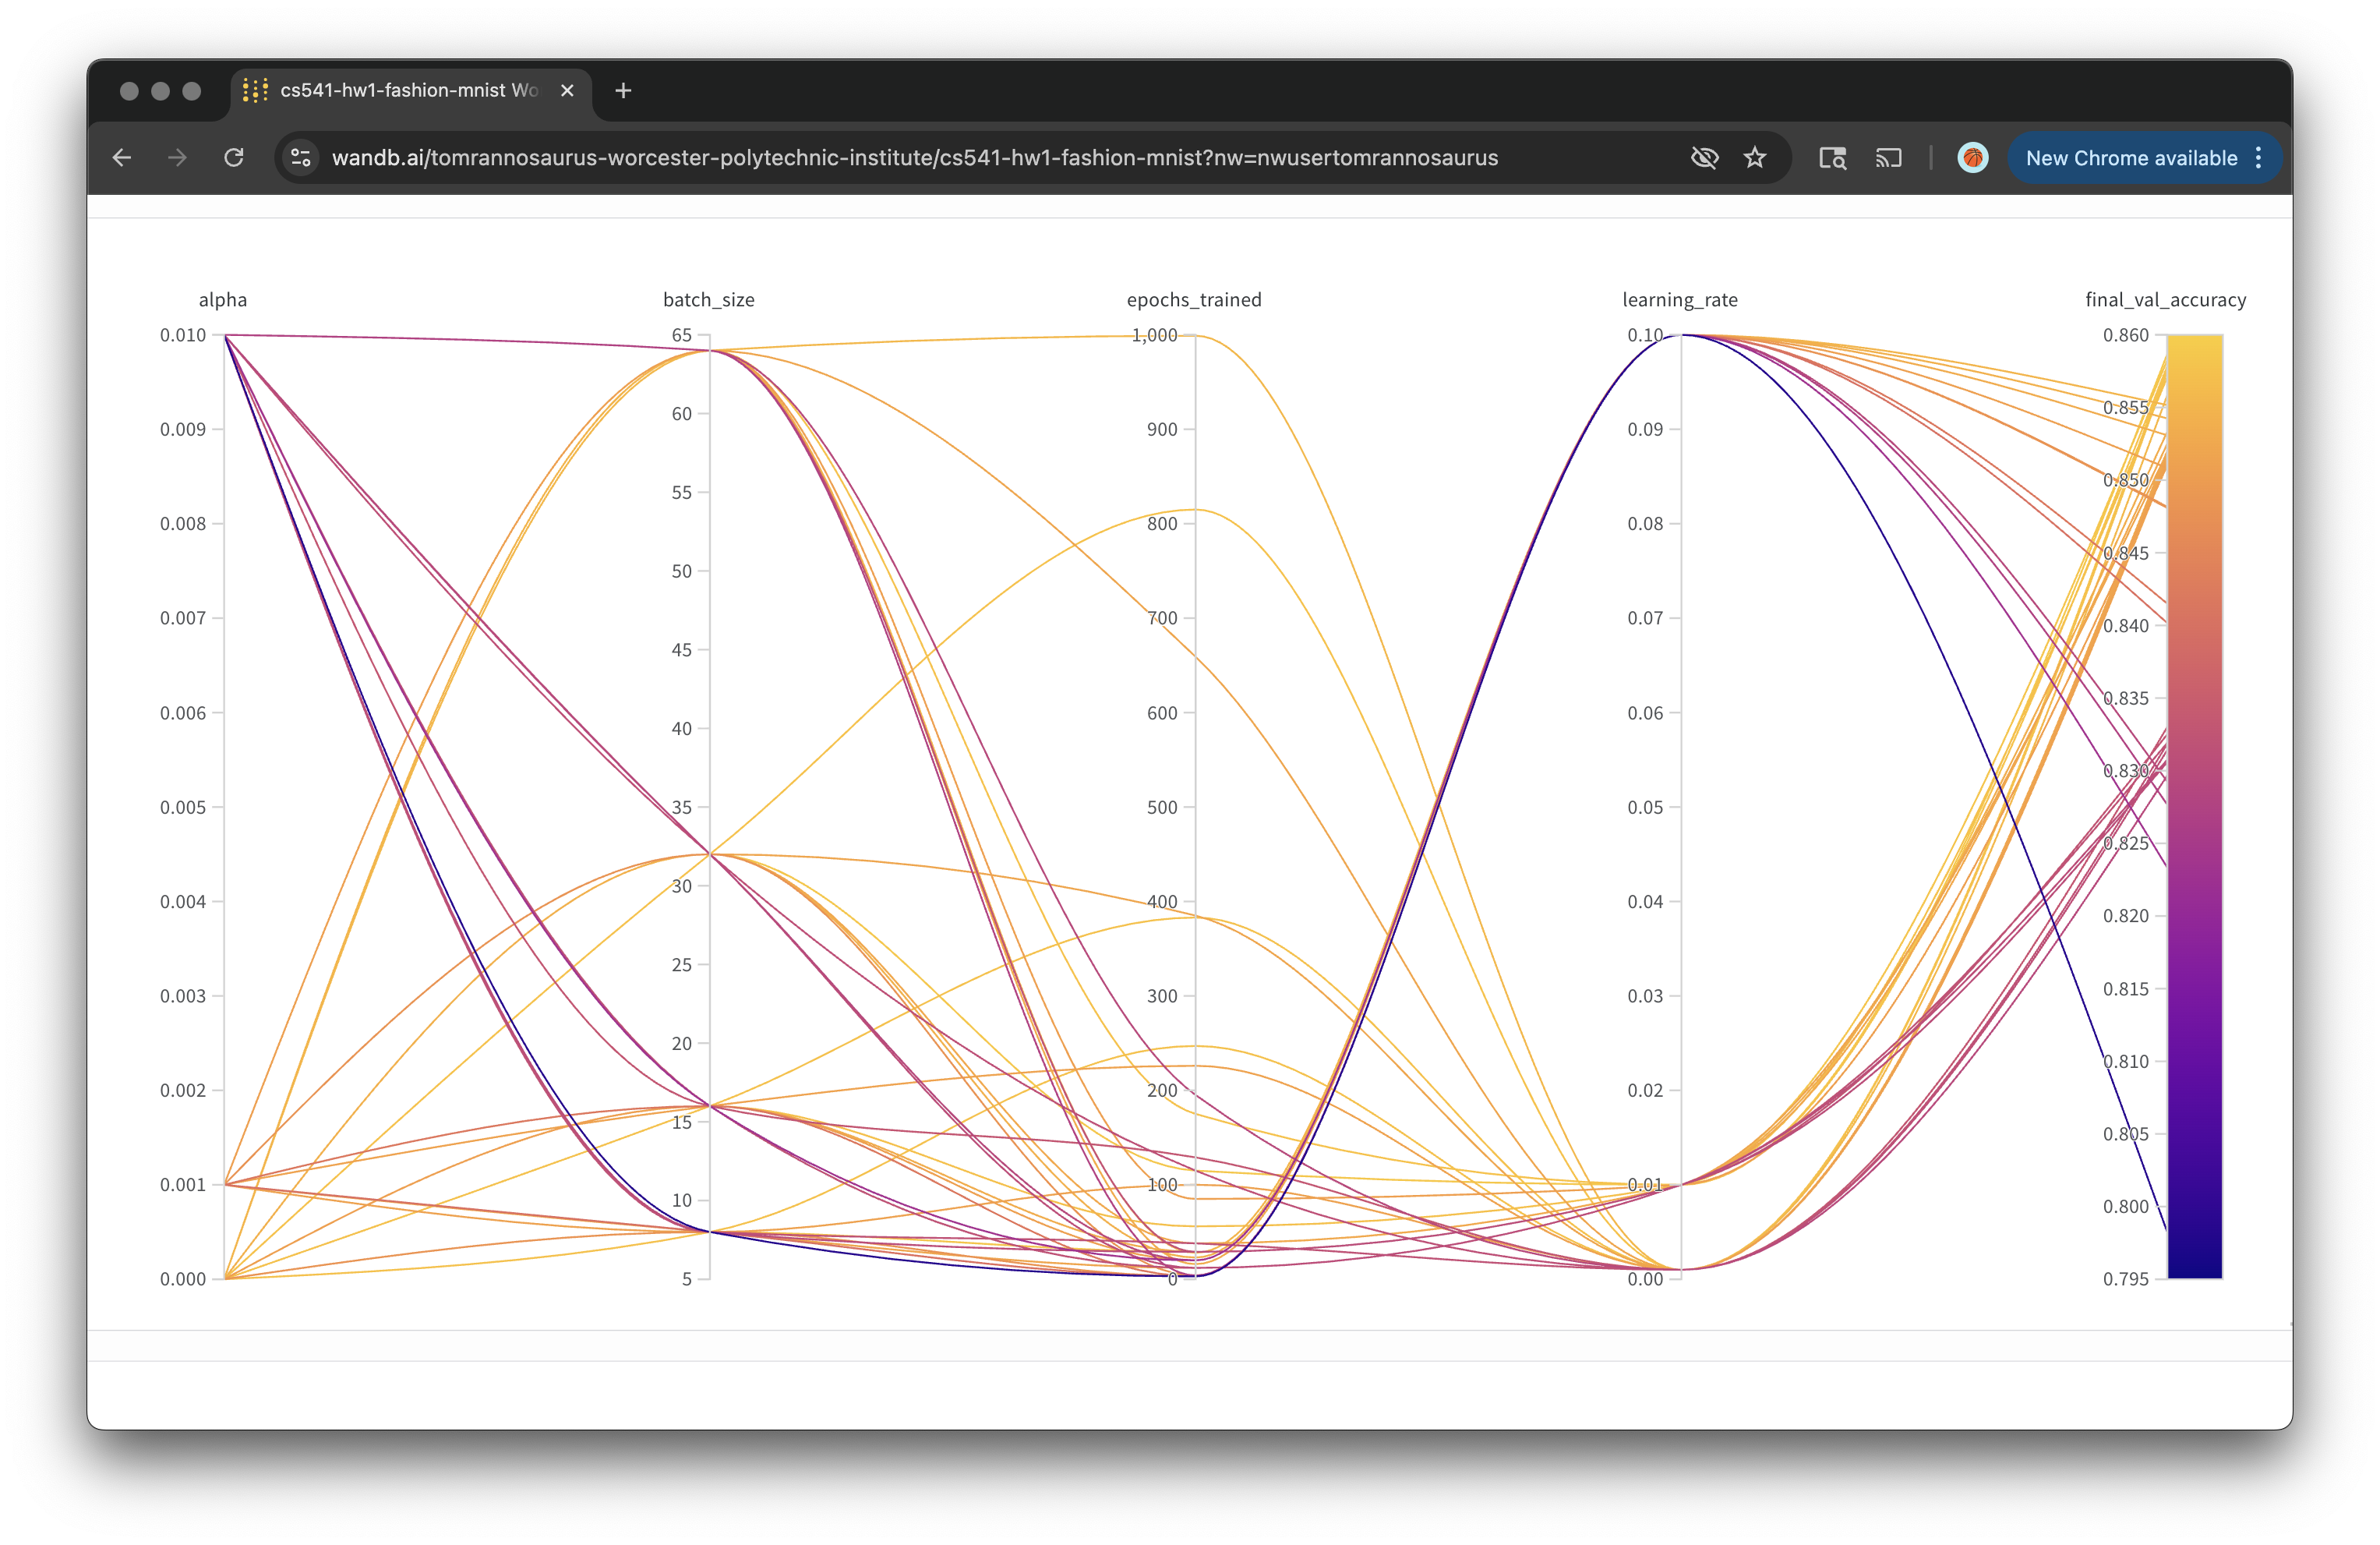
\includegraphics{wandb_parallel_coordinates_plot1.png}

}

\caption{Parallel Coordinates Plot: All Runs}

\end{figure}%%
\begin{figure}[H]

{\centering 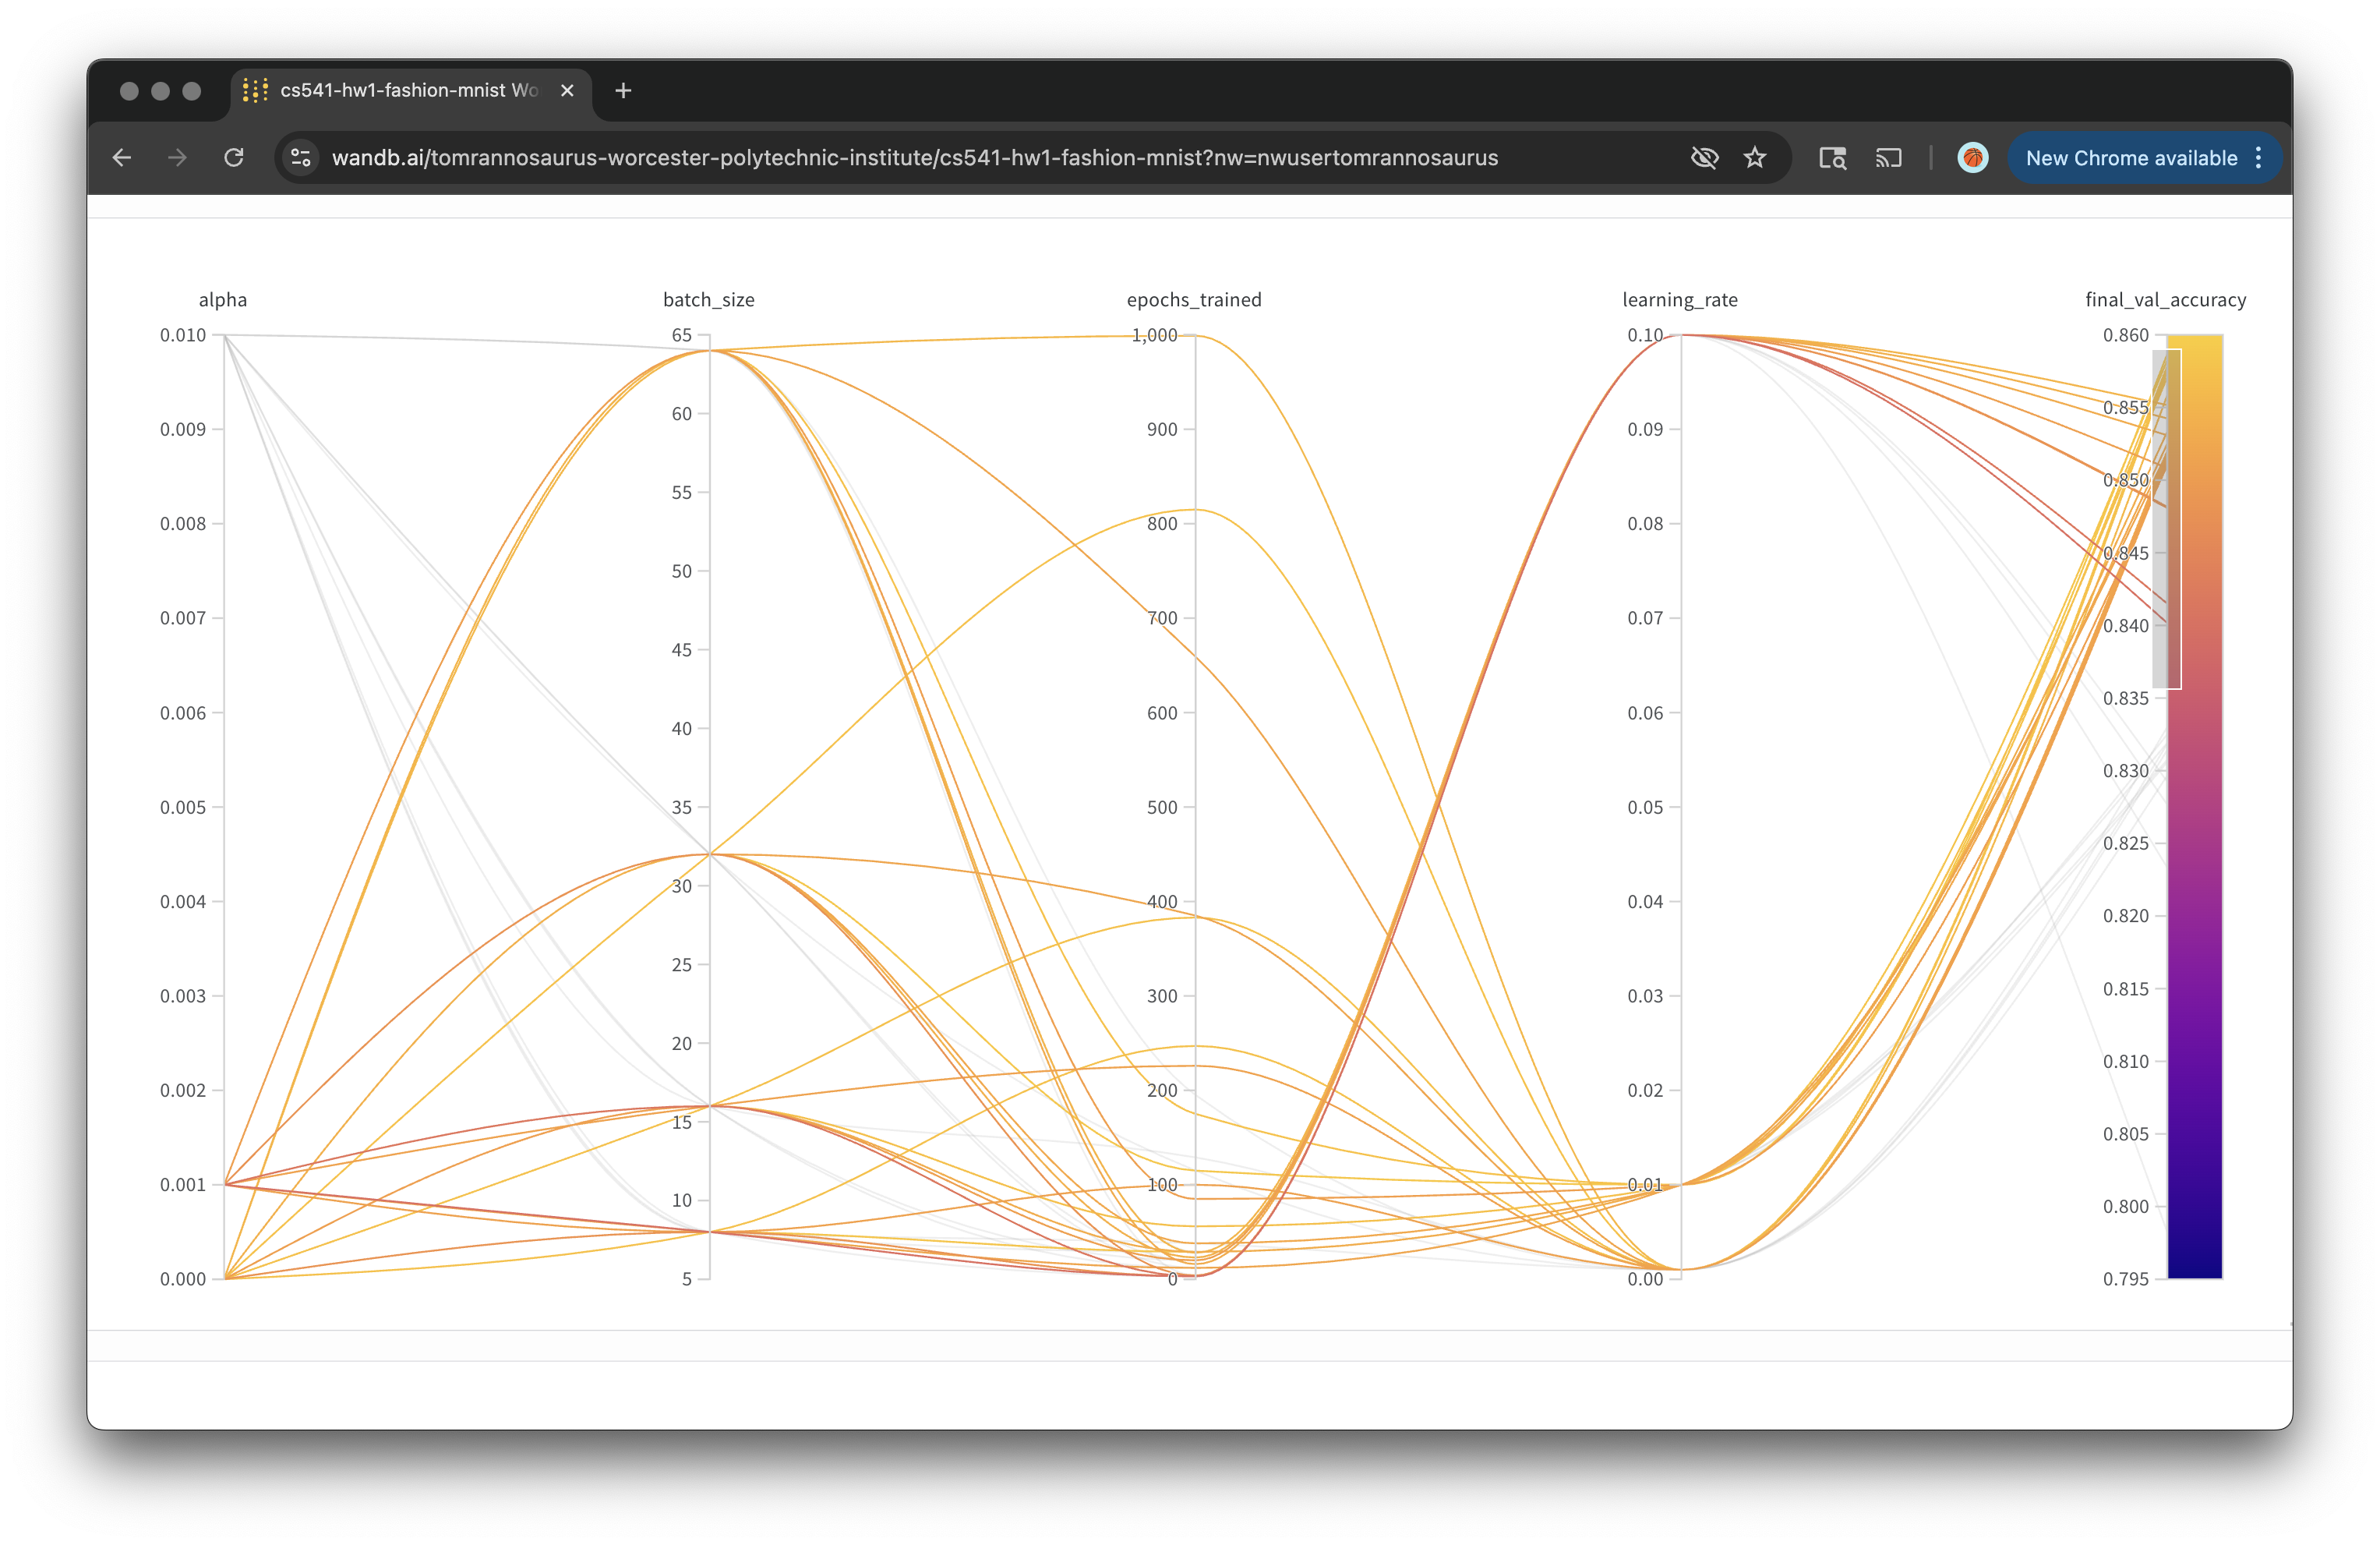
\includegraphics{wandb_parallel_coordinates_plot2.png}

}

\caption{Parallel Coordinates Plot: Filtered Top Runs 1}

\end{figure}%%
\begin{figure}[H]

{\centering 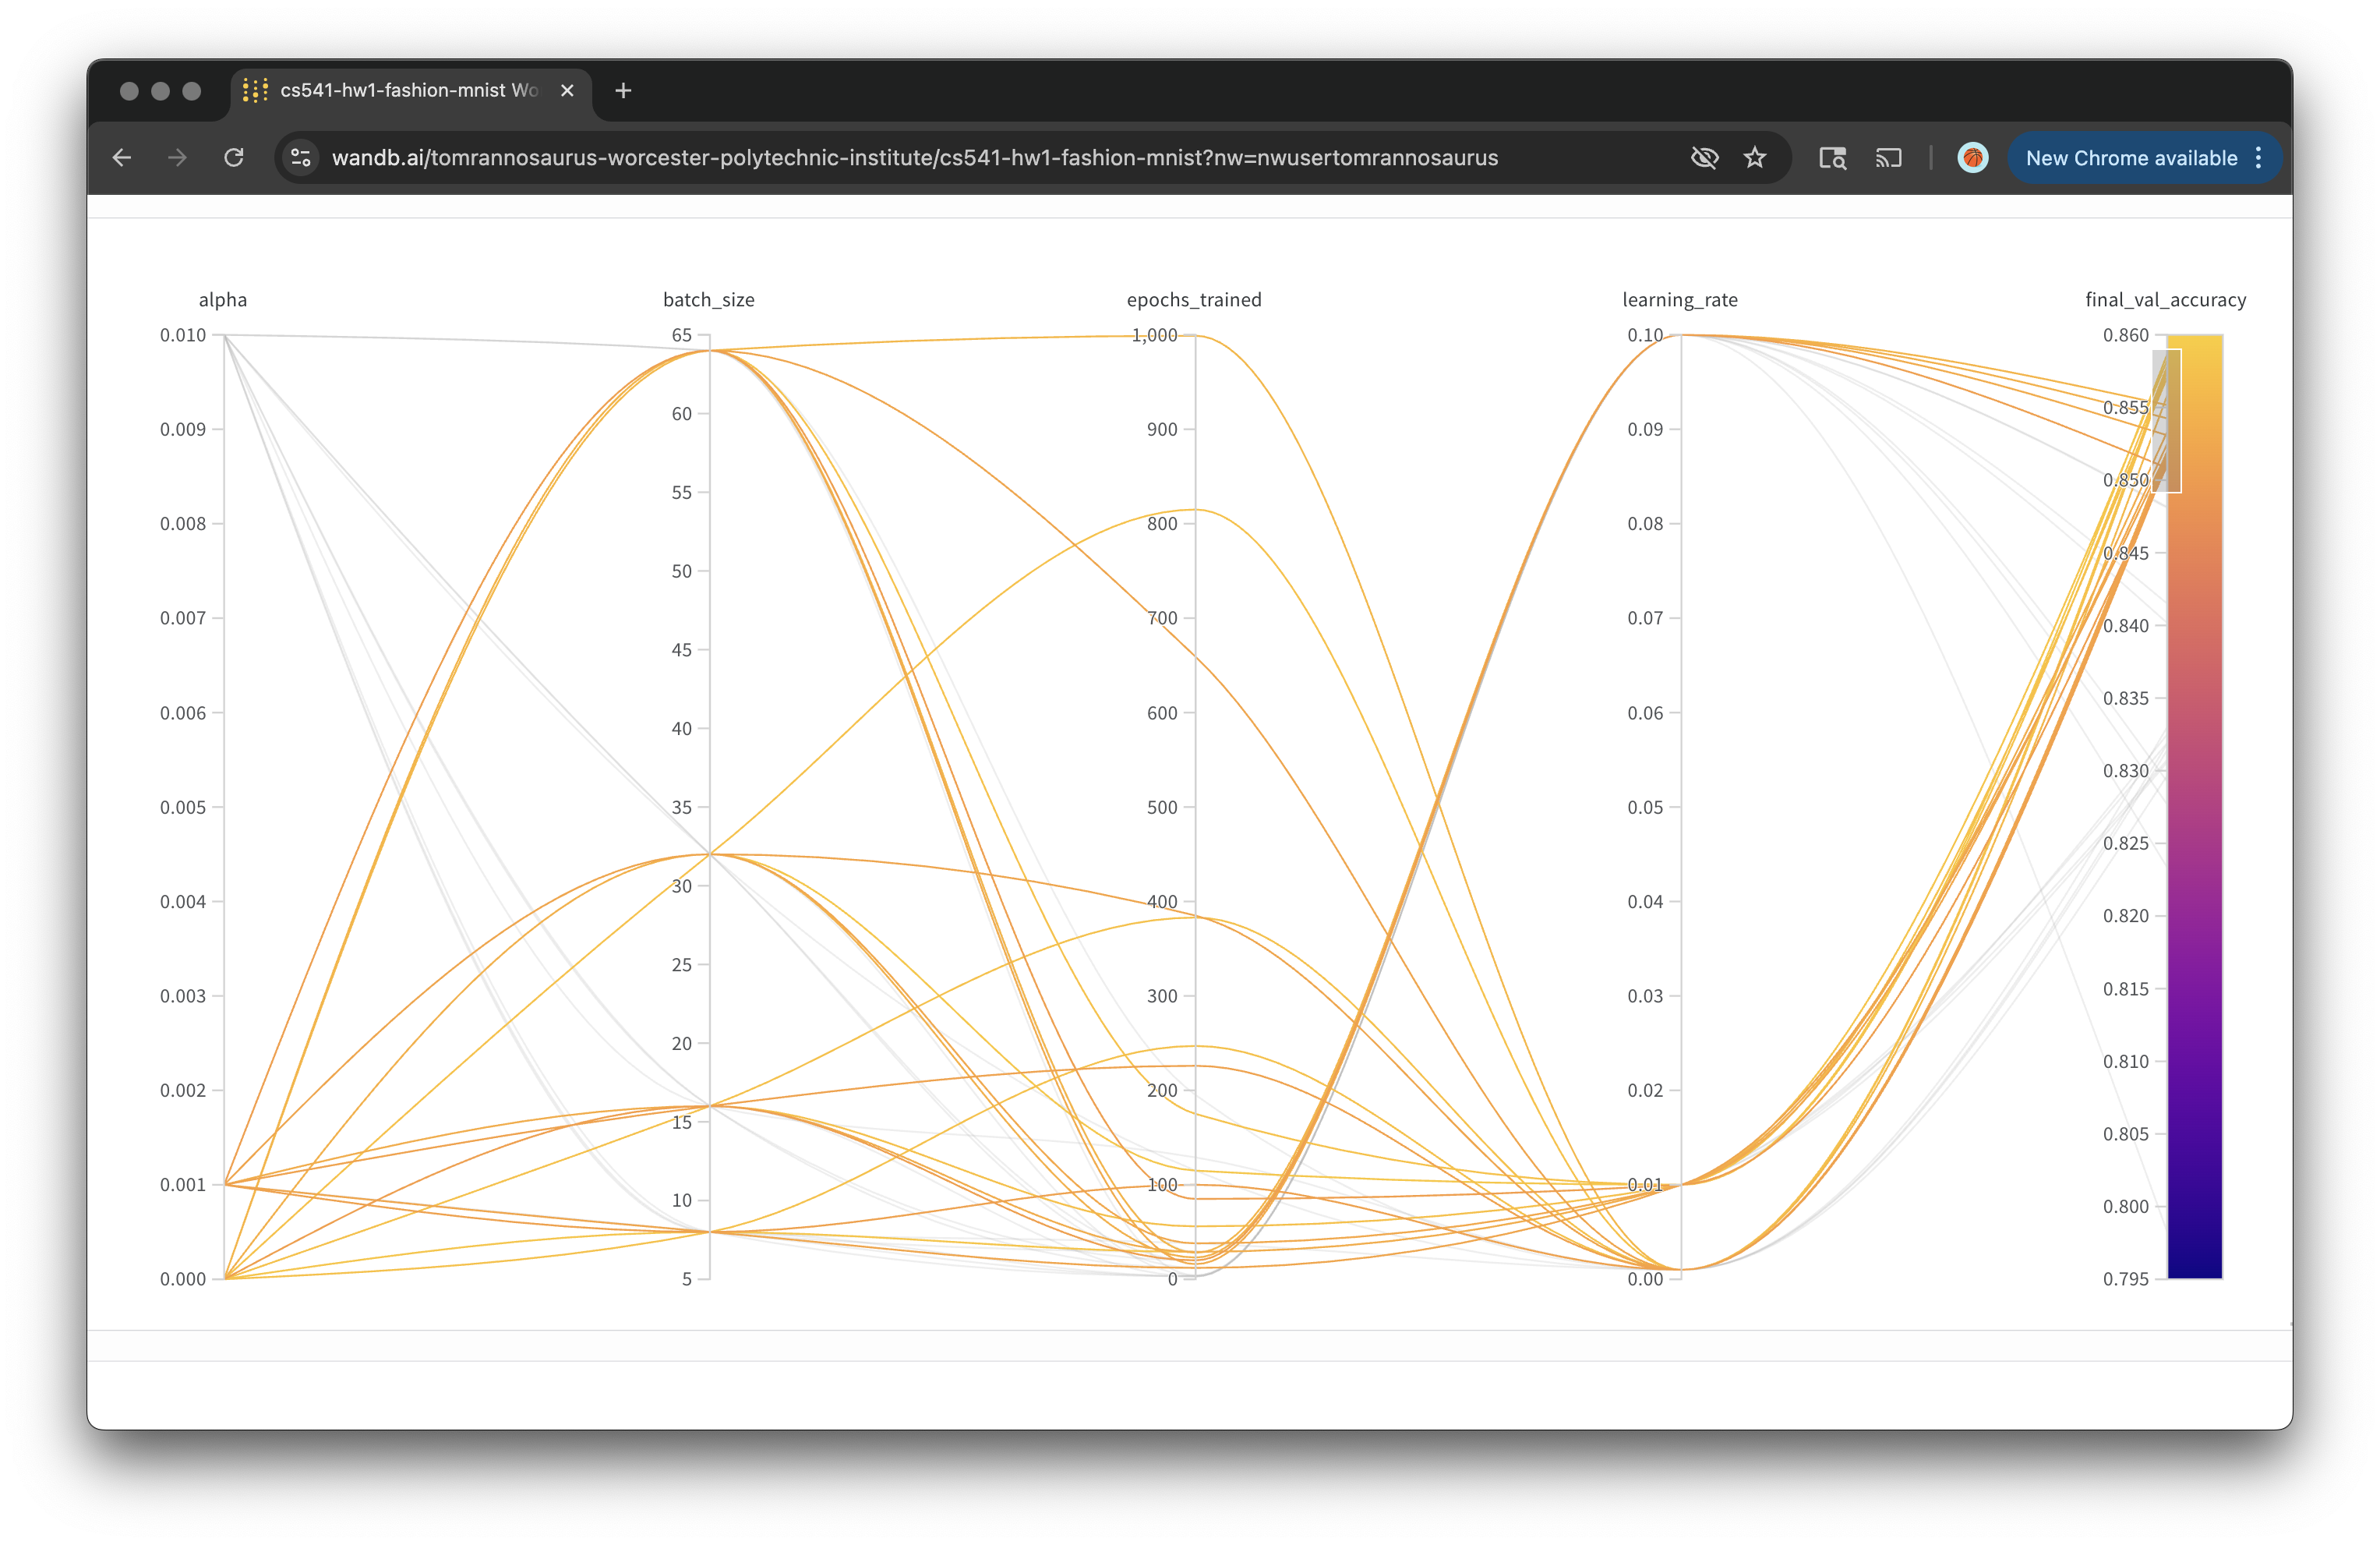
\includegraphics{wandb_parallel_coordinates_plot3.png}

}

\caption{Parallel Coordinates Plot: Filtered Top Runs 2}

\end{figure}%%
\begin{figure}[H]

{\centering 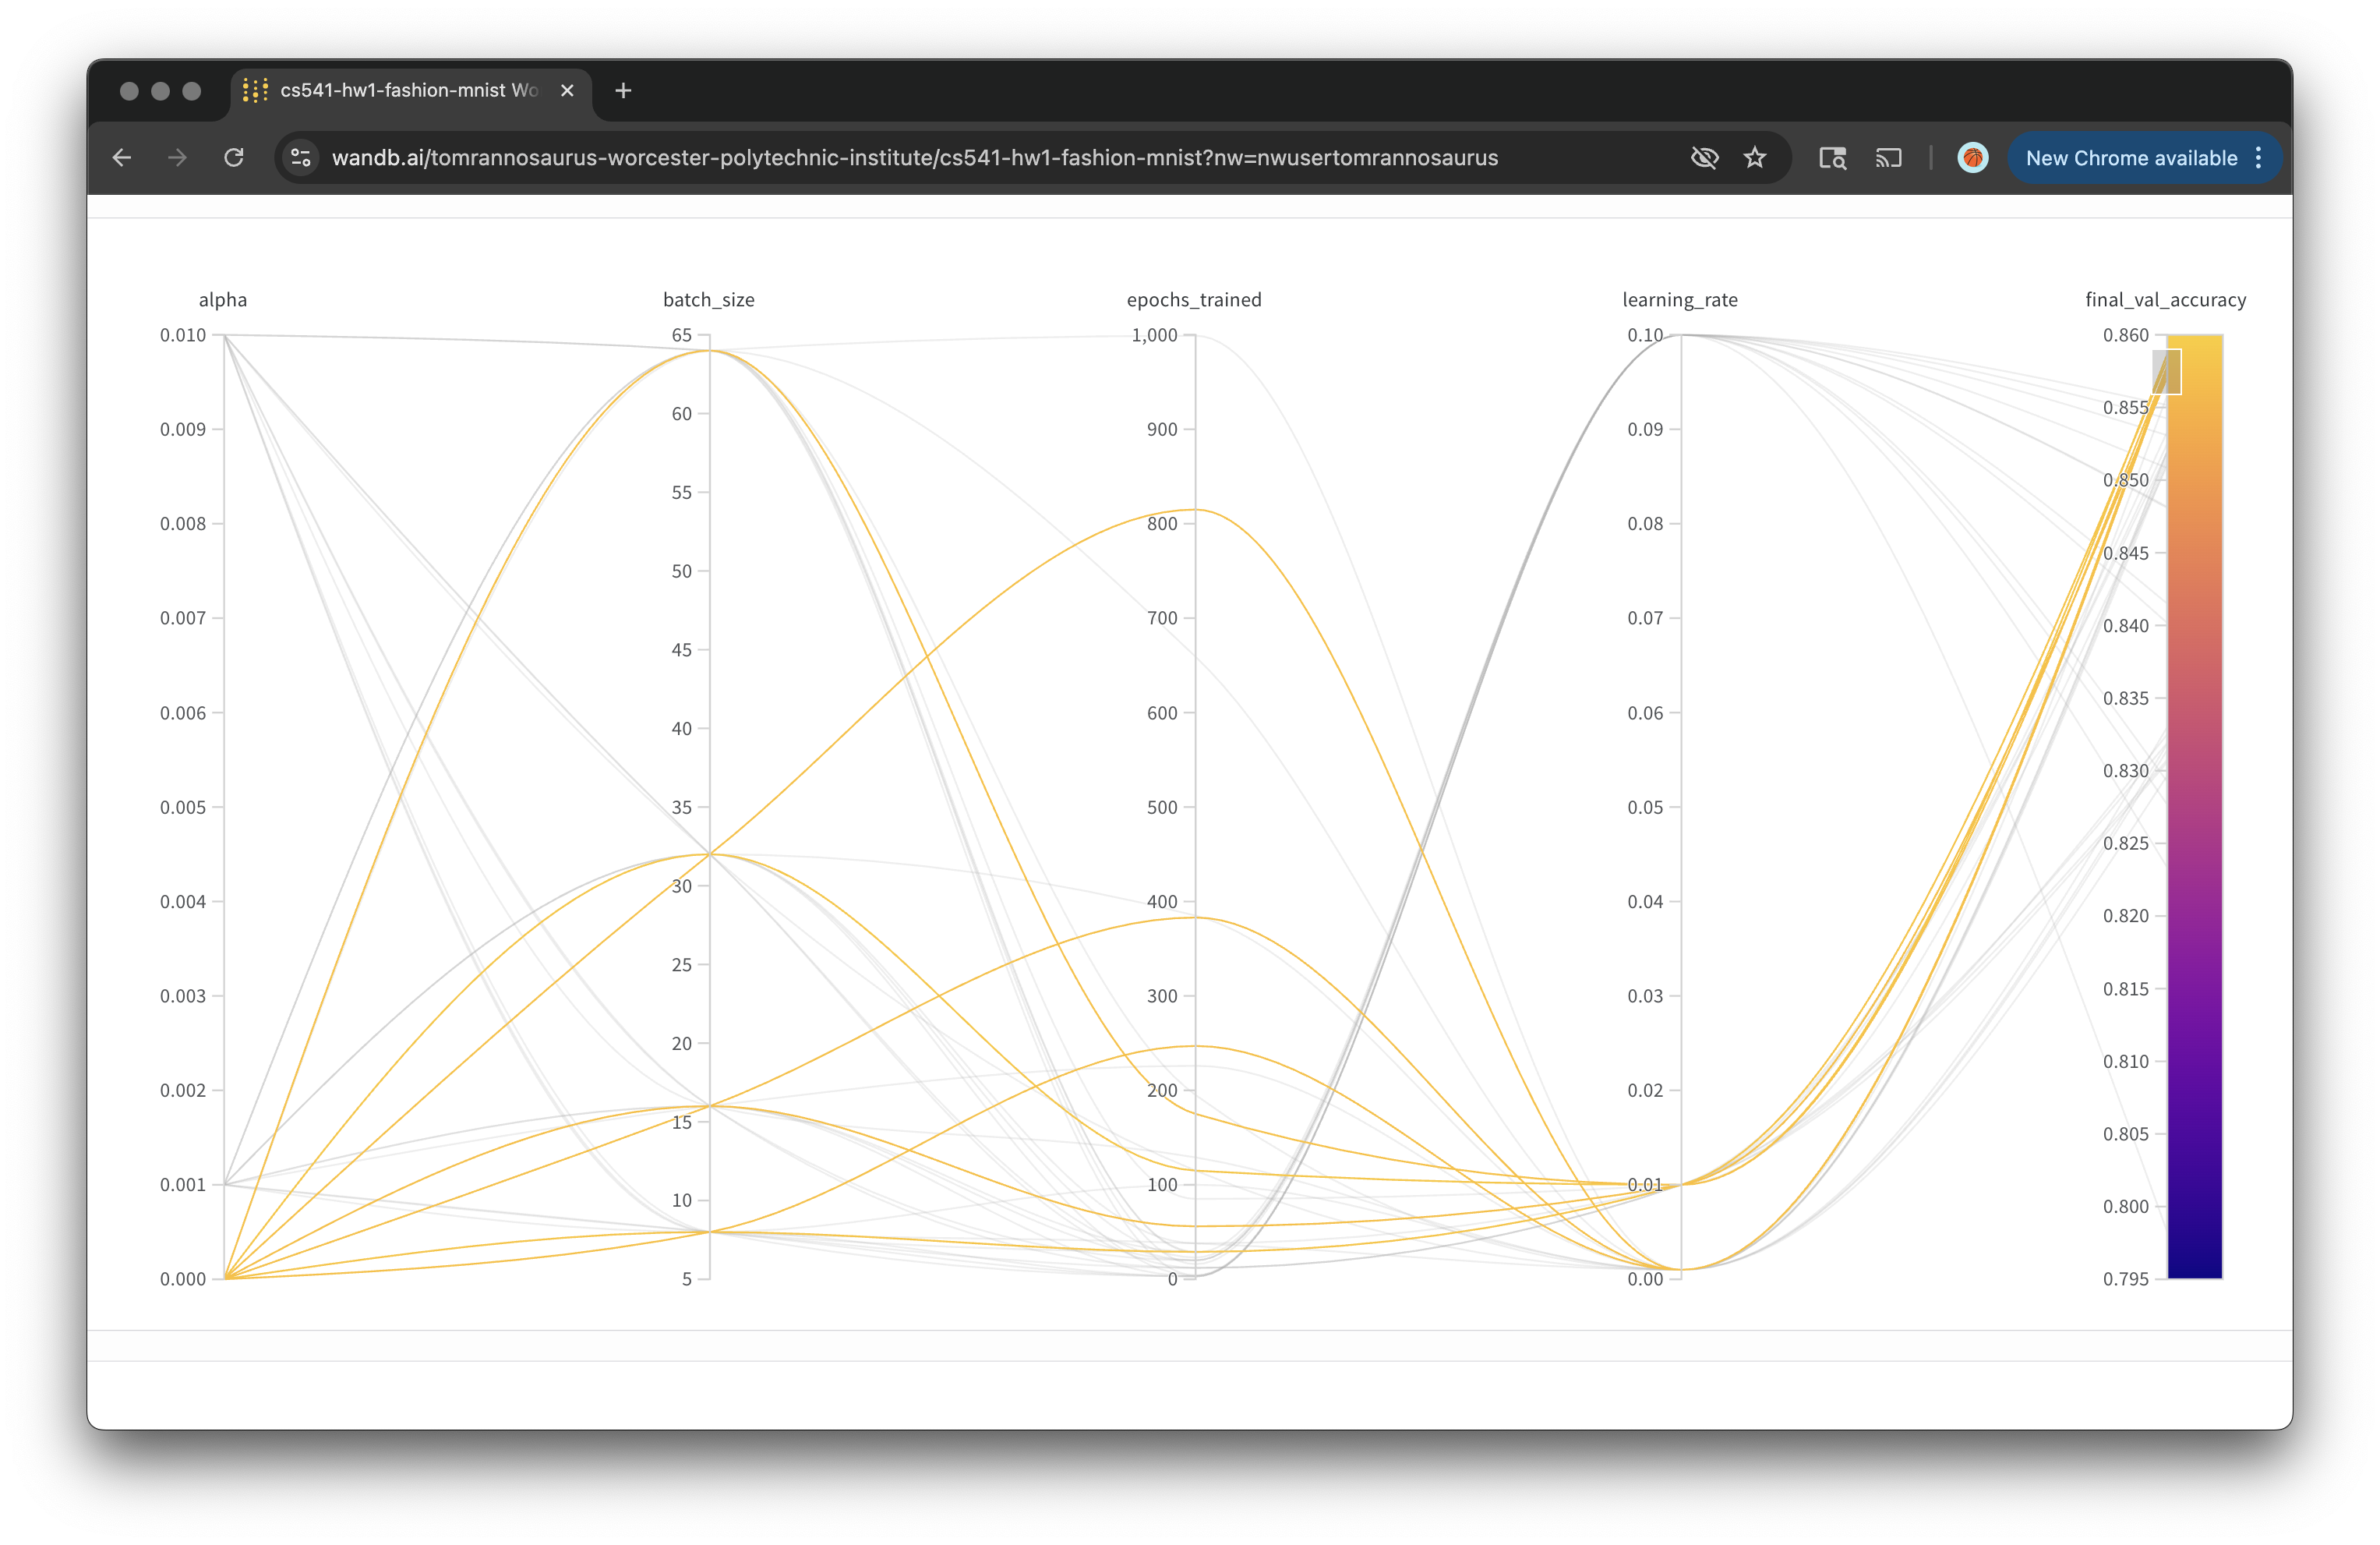
\includegraphics{wandb_parallel_coordinates_plot4.png}

}

\caption{Parallel Coordinates Plot: Filtered Top Runs 3}

\end{figure}%

\etwocol

Based on the parallel coordinates visualization, learning rate had the
most significant impact on validation accuracy. This is evident from the
performance stratification where all poor-performing runs converge
through learning rate 0.10, while high-performing runs pass through
0.01. Learning rates of 0.01 and sometimes 0.001 produced optimal
results; 0.10 consistently failed, likely due to optimization
instability. Regularization parameter alpha showed secondary effects,
with 0.010 correlating with decreased performance versus 0.000-0.001.
Batch size had minimal impact, with successful runs distributed across
all values.

The visualization provides clear advantages over tabular output. Pattern
recognition is immediate; the problematic learning rate 0.10 range would
be difficult to spot scanning 36 rows of numbers. Interaction effects
become visible, we see how learning rate 0.10 consistenly results in the
best final accuracy values, regardless of other settings. The plot gives
a unified view of the hyperparameter space.

\begin{center}\rule{0.5\linewidth}{0.5pt}\end{center}

\subsection{Problem 4: Implementing gradient computation via the
multivariate chain rule (linear case) {[}15
points{]}}\label{problem-4-implementing-gradient-computation-via-the-multivariate-chain-rule-linear-case-15-points}

Consider the two vector fields below taken from the Supplemental
Materials on Jacobian matrices and multivariate chain rule, slide 9:

\[
f\!\left(\begin{bmatrix} x_1 \\ x_2 \\ x_3 \end{bmatrix}\right) = x_1 - 2x_2 + \tfrac{x_3}{4}
\]

\[
g\!\left(\begin{bmatrix} x_1 \\ x_2 \end{bmatrix}\right) =
\begin{bmatrix}
x_1 + 2x_2 \\
x_2 \\
-x_1 + 3
\end{bmatrix}
\]

Let the initial input to \(g\) be

\[
x = \begin{bmatrix} -1 \\ 1 \end{bmatrix}.
\]

\begin{center}\rule{0.5\linewidth}{0.5pt}\end{center}

\begin{enumerate}
\def\labelenumi{\arabic{enumi}.}
\item
  Show how to represent each function as an affine transformation of the
  form \(Wx + b\). For function \(g\), denote the parameters by \(W_1\)
  and \(b_1\), whereas for function \(f\), denote the parameters by
  \(W_2\) and \(b_2\). {[}1 point{]}
\item
  Implement a python function \texttt{AffineTransformation(W,\ b,\ x)}
  that can be used to compute either function by taking as input two
  arrays of parameters \(W\) and \(b\) and a vector \(x\). {[}1 point{]}
\item
  Building on the previous function, implement a new function
  \texttt{Composition(L,\ x)} that calculates the composition of affine
  transformations represented as a list of pairs

  \[
  L = [(W_1, b_1), \ldots, (W_n, b_n)]
  \]

  and an initial vector \(x\). Use the following convention: the
  functions are applied from the smallest to the largest index. Return
  all the activation values (i.e., intermediate results) as a list
  variable

  \[
  z = (z_1, \ldots, z_n).
  \]

  {[}2 points{]}
\item
  How would you call the previous function to compute
  \((f \circ g)(x)\), for \(x = \begin{bmatrix} -1 \\ 1 \end{bmatrix}\)?
  Return \textbf{ONLY} the final output. {[}1 point{]}
\item
  Given an affine transformation \(z_2 = f(z_1)\) parameterized by
  \(W_2\) and \(b_2\), derive {[}2 points{]}:

  \[
  \frac{\partial z_2}{\partial \operatorname{vec}[W_2]}(z_1) \quad \text{and} \quad \frac{\partial z_2}{\partial b_2}(z_1).
  \]
\item
  Write equations for: {[}1 point{]}

  \[
  \frac{\partial (f \circ g)}{\partial z_1}(x)
  \]
\item
  For some scalar function \(y = (f \circ g)(x)\), where \(z = g(x)\) is
  an affine transformation parameterized by \(W_{n \times m}\) and
  \(b_{n \times 1}\), we know that

  \[
  \nabla_W y = \operatorname{unvec}\left[\frac{\partial y}{\partial z} \frac{\partial z}{\partial \operatorname{vec}[W]}\right]
  \]

  Last, if

  \[
  \frac{\partial y}{\partial z} = p^\top,
  \]

  then
\end{enumerate}

\[
\nabla_W y = p x^\top.
\]

Using the multivariate chain rule, write equations for: {[}2 points{]}

\[
\frac{\partial (f \circ g)}{\partial b_1} \quad \text{and} \quad \nabla_{W_1} (f \circ g)(x)
\]

\begin{center}\rule{0.5\linewidth}{0.5pt}\end{center}

\begin{enumerate}
\def\labelenumi{\arabic{enumi}.}
\setcounter{enumi}{7}
\item
  Using the list of parameters \(L\), the input vector \(x\) and all the
  activation values \(z\) obtained from the Composition, implement a
  function \texttt{ComputeGradients(L,x,z)} that returns the gradients
  of \(z_n\) (a scalar) for all the parameters in \(L\), i.e.,

  \[
  \nabla_{b_i} z_n = \left(\frac{\partial z_n}{\partial b_i}\right)^\top, \quad \nabla_{W_i} z_n.
  \]

  To earn full marks, the solution should apply to any \(n \geq 2\).
  {[}5 points{]}
\end{enumerate}

\begin{center}\rule{0.5\linewidth}{0.5pt}\end{center}

\subsubsection{Answers}\label{answers-1}

\begin{enumerate}
\def\labelenumi{\arabic{enumi}.}
\tightlist
\item
\end{enumerate}

Function g (\(\mathbb{R}^{2} \rightarrow \mathbb{R}^{3}\))

\[g\begin{pmatrix}x_1\\x_2\end{pmatrix} = \begin{pmatrix}x_1 + 2x_2\\x_2\\-x_1 + 3\end{pmatrix} = \begin{pmatrix}1 \cdot x_1 + 2 \cdot x_2 + 0\\0 \cdot x_1 + 1 \cdot x_2 + 0\\(-1) \cdot x_1 + 0 \cdot x_2 + 3\end{pmatrix}\]

\[= \begin{pmatrix}1 & 2\\0 & 1\\-1 & 0\end{pmatrix}\begin{pmatrix}x_1\\x_2\end{pmatrix} + \begin{pmatrix}0\\0\\3\end{pmatrix}\]

\[\mathbf{W_1} = \begin{pmatrix}1 & 2\\0 & 1\\-1 & 0\end{pmatrix} \in \mathbb{R}^{3 \times 2}, \quad \mathbf{b_1} = \begin{pmatrix}0\\0\\3\end{pmatrix} \in \mathbb{R}^3\]

Function f: (\(\mathbb{R}^{3} \rightarrow \mathbb{R}^{1}\))

\[f\begin{pmatrix}x_1\\x_2\\x_3\end{pmatrix} = x_1 - 2x_2 + \frac{x_3}{4} = \begin{pmatrix}1 & -2 & \frac{1}{4}\end{pmatrix}\begin{pmatrix}x_1\\x_2\\x_3\end{pmatrix} + 0\]

\[\mathbf{W_2} = \begin{pmatrix}1 & -2 & \frac{1}{4}\end{pmatrix} \in \mathbb{R}^{1 \times 3}, \quad b_2 = 0 \in \mathbb{R}\]

\begin{enumerate}
\def\labelenumi{\arabic{enumi}.}
\setcounter{enumi}{1}
\tightlist
\item
\end{enumerate}

\begin{Shaded}
\begin{Highlighting}[]
\KeywordTok{def}\NormalTok{ AffineTransformation(W, b, x):}
    \ControlFlowTok{return}\NormalTok{ W }\OperatorTok{@}\NormalTok{ x }\OperatorTok{+}\NormalTok{ b}
\end{Highlighting}
\end{Shaded}

\begin{enumerate}
\def\labelenumi{\arabic{enumi}.}
\setcounter{enumi}{2}
\tightlist
\item
\end{enumerate}

\begin{Shaded}
\begin{Highlighting}[]
\KeywordTok{def}\NormalTok{ Composition(L, x):}
\NormalTok{    z }\OperatorTok{=}\NormalTok{ [x]}
    \ControlFlowTok{for}\NormalTok{ W\_i, b\_i }\KeywordTok{in}\NormalTok{ L:}
\NormalTok{        z.append(W\_i }\OperatorTok{@}\NormalTok{ z[}\OperatorTok{{-}}\DecValTok{1}\NormalTok{] }\OperatorTok{+}\NormalTok{ b\_i)}
    \ControlFlowTok{return}\NormalTok{ z[}\DecValTok{1}\NormalTok{:]  }
\end{Highlighting}
\end{Shaded}

\begin{enumerate}
\def\labelenumi{\arabic{enumi}.}
\setcounter{enumi}{3}
\tightlist
\item
\end{enumerate}

\[(f \circ g)(\mathbf{x}) \text{ for } \mathbf{x} = \begin{pmatrix}-1\\1\end{pmatrix}\]

\[\mathbf{z_1} = g(\mathbf{x}) = \mathbf{W_1}\mathbf{x} + \mathbf{b_1}\]

\[= \begin{pmatrix}1 & 2\\0 & 1\\-1 & 0\end{pmatrix}\begin{pmatrix}-1\\1\end{pmatrix} + \begin{pmatrix}0\\0\\3\end{pmatrix}\]

\[= \begin{pmatrix}(1)(-1) + (2)(1)\\(0)(-1) + (1)(1)\\(-1)(-1) + (0)(1)\end{pmatrix} + \begin{pmatrix}0\\0\\3\end{pmatrix} = \begin{pmatrix}1\\1\\1\end{pmatrix} + \begin{pmatrix}0\\0\\3\end{pmatrix} = \begin{pmatrix}1\\1\\4\end{pmatrix}\]

\[z_2 = f(\mathbf{z_1}) = \mathbf{W_2}\mathbf{z_1} + b_2\]

\[= \begin{pmatrix}1 & -2 & \frac{1}{4}\end{pmatrix}\begin{pmatrix}1\\1\\4\end{pmatrix} + 0 = (1)(1) + (-2)(1) + \left(\frac{1}{4}\right)(4) = 0\]

\begin{enumerate}
\def\labelenumi{\arabic{enumi}.}
\setcounter{enumi}{4}
\tightlist
\item
\end{enumerate}

\begin{enumerate}
\def\labelenumi{(\alph{enumi})}
\tightlist
\item
  \(\frac{\partial z_2}{\partial \text{vec}[\mathbf{W_2}]}(\mathbf{z_1})\)
\end{enumerate}

\[\text{vec}_{\text{row}}[\mathbf{W_2}] = \begin{pmatrix}W_{2,1}\\W_{2,2}\\W_{2,3}\end{pmatrix} \in \mathbb{R}^3 \quad \text{(row-wise vec for } 1 \times 3 \text{ matrix)}\]

\[z_2 = W_{2,1}z_{1,1} + W_{2,2}z_{1,2} + W_{2,3}z_{1,3} + b_2\]

\[\frac{\partial z_2}{\partial W_{2,j}} = \frac{\partial}{\partial W_{2,j}}\left[\sum_{k=1}^3 W_{2,k}z_{1,k} + b_2\right] = z_{1,j}\]

\[\frac{\partial z_2}{\partial \text{vec}[\mathbf{W_2}]} = \begin{pmatrix}z_{1,1} & z_{1,2} & z_{1,3}\end{pmatrix} = \mathbf{z_1}^T \in \mathbb{R}^{1 \times 3}\]

\begin{enumerate}
\def\labelenumi{(\alph{enumi})}
\setcounter{enumi}{1}
\tightlist
\item
  \(\frac{\partial z_2}{\partial b_2}(\mathbf{z_1})\)
\end{enumerate}

\[\frac{\partial z_2}{\partial b_2} = \frac{\partial}{\partial b_2}[\mathbf{W_2}\mathbf{z_1} + b_2] = 1\]

\begin{enumerate}
\def\labelenumi{\arabic{enumi}.}
\setcounter{enumi}{5}
\tightlist
\item
\end{enumerate}

\(\frac{\partial(f \circ g)}{\partial \mathbf{z_1}}(\mathbf{x})\):

\[\frac{\partial z_2}{\partial z_{1,i}} = \frac{\partial}{\partial z_{1,i}}\left[\sum_{j=1}^3 W_{2,j}z_{1,j} + b_2\right] = W_{2,i}\]

\[\frac{\partial(f \circ g)}{\partial \mathbf{z_1}} = \begin{pmatrix}W_{2,1}\\W_{2,2}\\W_{2,3}\end{pmatrix} = \mathbf{W_2}^T = \begin{pmatrix}1\\-2\\\frac{1}{4}\end{pmatrix} \in \mathbb{R}^{3 \times 1}\]

\begin{enumerate}
\def\labelenumi{\arabic{enumi}.}
\setcounter{enumi}{6}
\tightlist
\item
\end{enumerate}

\begin{enumerate}
\def\labelenumi{(\alph{enumi})}
\tightlist
\item
  \(\frac{\partial(f \circ g)}{\partial \mathbf{b_1}}\)
\end{enumerate}

\[\mathbf{z_1} = \mathbf{W_1}\mathbf{x} + \mathbf{b_1} \quad \rightarrow \quad \frac{\partial z_{1,k}}{\partial b_{1,i}} = \delta_{ki}\]

\[\frac{\partial z_2}{\partial b_{1,i}} = \sum_{k=1}^3 \frac{\partial z_2}{\partial z_{1,k}} \cdot \frac{\partial z_{1,k}}{\partial b_{1,i}} = \sum_{k=1}^3 W_{2,k} \cdot \delta_{ki} = W_{2,i}\]

\[\frac{\partial(f \circ g)}{\partial \mathbf{b_1}} = \begin{pmatrix}W_{2,1}\\W_{2,2}\\W_{2,3}\end{pmatrix} = \mathbf{W_2}^T = \begin{pmatrix}1\\-2\\\frac{1}{4}\end{pmatrix} \in \mathbb{R}^{3 \times 1}\]

\begin{enumerate}
\def\labelenumi{(\alph{enumi})}
\setcounter{enumi}{1}
\tightlist
\item
  \(\nabla_{\mathbf{W_1}}(f \circ g)(\mathbf{x})\)
\end{enumerate}

\[\text{vec}_{\text{row}}[\mathbf{W_1}] = \begin{pmatrix}W_{11}\\W_{12}\\W_{21}\\W_{22}\\W_{31}\\W_{32}\end{pmatrix} \in \mathbb{R}^6 \quad \text{(stack rows sequentially)}\]

\[\mathbf{z_1} = \mathbf{W_1}\mathbf{x} + \mathbf{b_1} = \begin{pmatrix}W_{11}x_1 + W_{12}x_2 + b_{1,1}\\W_{21}x_1 + W_{22}x_2 + b_{1,2}\\W_{31}x_1 + W_{32}x_2 + b_{1,3}\end{pmatrix}\]

\[\frac{\partial z_{1,i}}{\partial W_{ij}} = \frac{\partial}{\partial W_{ij}}\left[\sum_{k=1}^2 W_{ik}x_k + b_{1,i}\right] = x_j\]

\[\frac{\partial \mathbf{z_1}}{\partial \text{vec}_{\text{row}}[\mathbf{W_1}]} = \begin{pmatrix}
\frac{\partial z_{1,1}}{\partial W_{11}} & \frac{\partial z_{1,1}}{\partial W_{12}} & \frac{\partial z_{1,1}}{\partial W_{21}} & \frac{\partial z_{1,1}}{\partial W_{22}} & \frac{\partial z_{1,1}}{\partial W_{31}} & \frac{\partial z_{1,1}}{\partial W_{32}}\\
\frac{\partial z_{1,2}}{\partial W_{11}} & \frac{\partial z_{1,2}}{\partial W_{12}} & \frac{\partial z_{1,2}}{\partial W_{21}} & \frac{\partial z_{1,2}}{\partial W_{22}} & \frac{\partial z_{1,2}}{\partial W_{31}} & \frac{\partial z_{1,2}}{\partial W_{32}}\\
\frac{\partial z_{1,3}}{\partial W_{11}} & \frac{\partial z_{1,3}}{\partial W_{12}} & \frac{\partial z_{1,3}}{\partial W_{21}} & \frac{\partial z_{1,3}}{\partial W_{22}} & \frac{\partial z_{1,3}}{\partial W_{31}} & \frac{\partial z_{1,3}}{\partial W_{32}}
\end{pmatrix}\]

\[= \begin{pmatrix}
x_1 & x_2 & 0 & 0 & 0 & 0\\
0 & 0 & x_1 & x_2 & 0 & 0\\
0 & 0 & 0 & 0 & x_1 & x_2
\end{pmatrix} \in \mathbb{R}^{3 \times 6}\]

\[\frac{\partial z_2}{\partial \text{vec}_{\text{row}}[\mathbf{W_1}]} = \frac{\partial z_2}{\partial \mathbf{z_1}} \cdot \frac{\partial \mathbf{z_1}}{\partial \text{vec}_{\text{row}}[\mathbf{W_1}]} \quad \text{(chain rule)}\]

\[= \mathbf{W_2} \begin{pmatrix}
x_1 & x_2 & 0 & 0 & 0 & 0\\
0 & 0 & x_1 & x_2 & 0 & 0\\
0 & 0 & 0 & 0 & x_1 & x_2
\end{pmatrix}\]

\[= \begin{pmatrix}W_{2,1} & W_{2,2} & W_{2,3}\end{pmatrix} \begin{pmatrix}
x_1 & x_2 & 0 & 0 & 0 & 0\\
0 & 0 & x_1 & x_2 & 0 & 0\\
0 & 0 & 0 & 0 & x_1 & x_2
\end{pmatrix}\]

\[= \begin{pmatrix}W_{2,1}x_1 & W_{2,1}x_2 & W_{2,2}x_1 & W_{2,2}x_2 & W_{2,3}x_1 & W_{2,3}x_2\end{pmatrix}\]

\[\nabla_{\mathbf{W_1}}(f \circ g) = \text{unvec}_{\text{row}}\left[\begin{pmatrix}W_{2,1}x_1\\W_{2,1}x_2\\W_{2,2}x_1\\W_{2,2}x_2\\W_{2,3}x_1\\W_{2,3}x_2\end{pmatrix}\right]_{3 \times 2}\]

\[= \begin{pmatrix}W_{2,1}x_1 & W_{2,1}x_2\\W_{2,2}x_1 & W_{2,2}x_2\\W_{2,3}x_1 & W_{2,3}x_2\end{pmatrix} = \begin{pmatrix}W_{2,1}\\W_{2,2}\\W_{2,3}\end{pmatrix}\begin{pmatrix}x_1 & x_2\end{pmatrix} = \mathbf{W_2}^T \mathbf{x}^T \in \mathbb{R}^{3 \times 2}\]

Given Identity:

\[\text{If } \frac{\partial y}{\partial \mathbf{z}} = \mathbf{p}^T \text{ then } \nabla_{\mathbf{W}}y = \mathbf{p}\mathbf{x}^T \quad \text{(outer product)}\]

\begin{enumerate}
\def\labelenumi{\arabic{enumi}.}
\setcounter{enumi}{7}
\tightlist
\item
\end{enumerate}

\[\text{Given: } L = [(\mathbf{W_1}, \mathbf{b_1}), \ldots, (\mathbf{W_n}, \mathbf{b_n})], \quad \mathbf{x}, \quad \mathbf{z} = [\mathbf{z_1}, \ldots, \mathbf{z_n}]\]

\[\text{Forward pass: } \mathbf{z_0} = \mathbf{x}, \quad \mathbf{z_{i}} = \mathbf{W_i}\mathbf{z_{i-1}} + \mathbf{b_i}, \quad i = 1, \ldots, n\]

\[\text{Initialize: } \frac{\partial z_n}{\partial z_n} = 1 \quad \text{(scalar output)}\]

\[\text{Backward recursion: } \frac{\partial z_n}{\partial \mathbf{z_{i-1}}} = \frac{\partial z_n}{\partial \mathbf{z_i}} \cdot \frac{\partial \mathbf{z_i}}{\partial \mathbf{z_{i-1}}} = \frac{\partial z_n}{\partial \mathbf{z_i}} \cdot \mathbf{W_i}^T\]

\[\nabla_{\mathbf{W_i}} z_n = \left(\frac{\partial z_n}{\partial \mathbf{z_i}}\right) \mathbf{z_{i-1}}^T \quad \text{(apply key identity with } \mathbf{p} = \frac{\partial z_n}{\partial \mathbf{z_i}}, \; \mathbf{x} = \mathbf{z_{i-1}}\text{)}\]

\[\nabla_{\mathbf{b_i}} z_n = \frac{\partial z_n}{\partial \mathbf{z_i}}\]

\begin{Shaded}
\begin{Highlighting}[]
\KeywordTok{def}\NormalTok{ ComputeGradients(L, x, z):}
\NormalTok{    n }\OperatorTok{=} \BuiltInTok{len}\NormalTok{(L)}
\NormalTok{    z\_full }\OperatorTok{=}\NormalTok{ [x] }\OperatorTok{+}\NormalTok{ z}
    
\NormalTok{    grad\_z }\OperatorTok{=} \DecValTok{1}
\NormalTok{    gradients }\OperatorTok{=}\NormalTok{ []}
    
    \ControlFlowTok{for}\NormalTok{ i }\KeywordTok{in} \BuiltInTok{range}\NormalTok{(n, }\DecValTok{0}\NormalTok{, }\OperatorTok{{-}}\DecValTok{1}\NormalTok{):}
\NormalTok{        W\_i, b\_i }\OperatorTok{=}\NormalTok{ L[i}\OperatorTok{{-}}\DecValTok{1}\NormalTok{]}
\NormalTok{        grad\_b\_i }\OperatorTok{=}\NormalTok{ grad\_z}
\NormalTok{        grad\_W\_i }\OperatorTok{=}\NormalTok{ grad\_z }\OperatorTok{@}\NormalTok{ z\_full[i}\OperatorTok{{-}}\DecValTok{1}\NormalTok{].T}
\NormalTok{        gradients.append((grad\_W\_i, grad\_b\_i))}
\NormalTok{        grad\_z }\OperatorTok{=}\NormalTok{ W\_i.T }\OperatorTok{@}\NormalTok{ grad\_z  }\CommentTok{\# propagate backward}
    
    \ControlFlowTok{return} \BuiltInTok{list}\NormalTok{(}\BuiltInTok{reversed}\NormalTok{(gradients))}
\end{Highlighting}
\end{Shaded}

\[\text{General formula for } n \geq 2\text{:}\]

\[\nabla_{\mathbf{W_i}}z_n = \left(\prod_{j=n}^{i+1} \mathbf{W_j}^T\right)^T \mathbf{z_{i-1}}^T\]

\[\nabla_{\mathbf{b_i}}z_n = \left(\prod_{j=n}^{i+1} \mathbf{W_j}^T\right)^T\]

\begin{center}\rule{0.5\linewidth}{0.5pt}\end{center}

\subsection{Submission}\label{submission}

Submit one PDF file that includes your notes for the theoretical
problems (scanned or typed) and screenshots of your code for the
programming problems. All material in the submitted PDF must be
presented in a clear and readable format.

If you are working as part of a group, then indicate the members on
canvas: \url{https://canvas.wpi.edu/courses/76771/groups\#tab-14853}.
Once you do that, be aware that any submission from a team member will
overwrite an existing one.

\begin{center}\rule{0.5\linewidth}{0.5pt}\end{center}

\subsection{Teamwork}\label{teamwork}

You may complete this homework assignment either individually or in
teams up to 2 people.

\url{https://canvas.wpi.edu/courses/76771/groups\#tab-14853}
\url{https://canvas.wpi.edu/courses/76771/groups\#tab-14853}




\end{document}
